%%%%%%%%%%%%%%%%%%%%%%%%%%%%%%%
\chapter{Data sets and simulated samples}
\label{ch:dataAndSim}
%%%%%%%%%%%%%%%%%%%%%%%%%%%%%%%

The simulation of pp collisions is usually performed by means of Monte Carlo (MC) event generators, providing an accurate modelling of the event kinematics and topology at parton and hadron level.
The hard inelastic scattering has to be fully calculated: from the hard interaction between the partons inside the protons, where perturbative QCD calculations (\FIXME{point to theory}) can be used, to the formation of particle jets from the outgoing partons.
Furthermore, it is fundamental to understand the exact response of the detector to the outgoing particles produced in pp collisions. 
Consequently, the stable outgoing particles are fed to a full detector simulation that models the interaction of those particles with the detector material and the corresponding detector response.
The raw detector data are then subject to the same reconstruction algorithms that are also used for real data.
In this chapter, MC event generators are described in detail, followed by a brief description of the CMS detector simulation.
Finally, few details are given in the last section on the pp collision data sets used to perform the searches described in this thesis.

%%%%%%%%%%%%%%%%%%%%%%%%%%%%%%%
\section{Simulation of proton-proton collisions}
%%%%%%%%%%%%%%%%%%%%%%%%%%%%%%%

%%%%
\subsection{Monte Carlo event generators}
%%%%

The generation of hard inelastic pp collisions is factorized into different steps ordered by the timescale on which they happen, as illustrated in Fig.~\ref{fig:MCgenSteps}, and described in the following.\\

\begin{figure}[!htb]
\centering
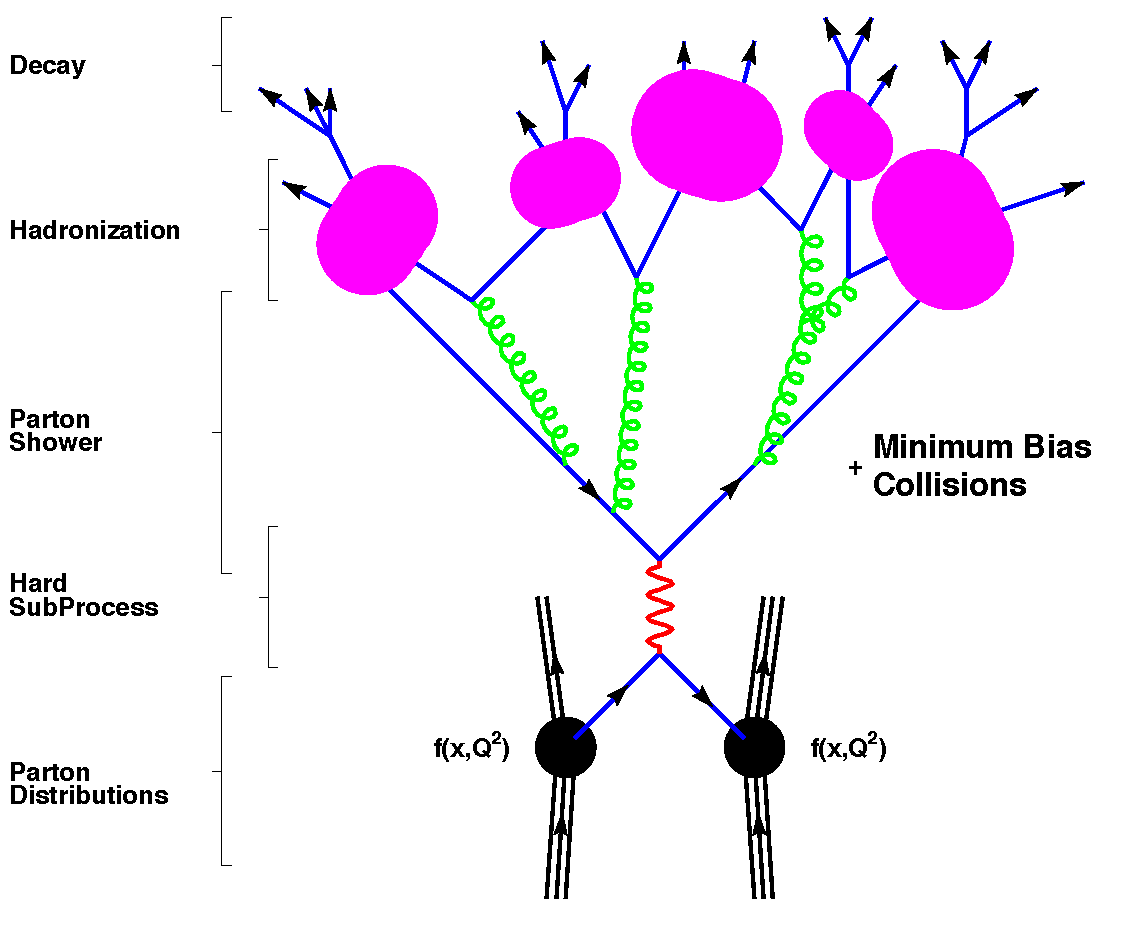
\includegraphics[width=0.8\textwidth]{\chfive/f_shg_event.pdf}
\caption{Steps of Monte Carlo event generation as described in the text evolving in time from bottom to top~\cite{Dobbs:2004qw}.}
\label{fig:MCgenSteps}
\end{figure}

The basis of theoretical event generation at the LHC is a parametrisation of the incoming partons (quarks, anti-quarks and gluons) stemming from the proton, which is given by the parton density functions (PDF).
They describe the probability to find a quark or gluon with a given proton momentum fraction $x$ in the pp collision taking place at the LHC.
In QCD the PDFs depend on a factorization scale $\mu^2_F$ at which the proton is probed.
All interactions between quarks and gluons happening at scales below the scale $\mu^2_F$ are absorbed into the PDFs. Therefore at small $\mu^2_F$ the proton is observed basically as a combination of its
three valence quarks $uud$. At higher scales, however, it is dominated by sea quarks and gluons.

A collision between two partons, one from each side, gives the hard process of interest, which can be due to physics within or beyond the standard model.
Using the incoming partons as input, the simulation of the hard process is performed by the event generator.
It produces hypothetical events with the distributions and rates predicted by theory based on the cross section formulae of the physics process of interest.
Using the cross section formula the phase space is sampled and candidate events are defined by choosing values for the degrees of freedom from a uniformly distributed random number generator.

The cross section can be calculated by means of the so called \textit{factorization theorem}~\cite{Collins:1987pm}.
According to the theorem, the hadron itself is described by the whole particle composition interacting on a soft binding energy scale,
whereas the collisions occur between the partons on a hard energy scale with large transverse momenta.
The cross section for the process is then given by the convolution of the PDF $f_i(x,Q^2)$, integrated over the proton momentum fraction $x$, for the colliding protons (A, B) at an energy scale $Q^2$,
and the hard parton-parton cross sections $\hat{\sigma}_{ij} \to X$ for all combinations of two partons i and j:
%The cross section for two colliding protons can be seen as the convolution of the cross section $\hat{\sigma}_{ij} \rightarrow X$ for two interacting partons $i$ and $j$ inside the protons,
%with the parton distribution functions $f_1(x_1, Q^2)$, $f_2(x_2, Q^2)$ (PDF), integrated over the Bjorken variables $x_1$, $x_2$,
%defined as the fraction of the 4-momentum carried out by the two partons inside the proton during the collision

\begin{equation}
\sigma(AB \to X) = \sum_{q,g=0}^{n} \alpha_S^n(\mu_R^2)\sum_{ij}\int dx_i dx_j f_{i,A}(x_i,\mu_F^2) f_{j,B}(x_j,\mu_F^2) \cdot \hat{\sigma}^{(n)}_{ij\to X}(s;x_i,x_j,\mu_R^2,\mu_F^2).
\end{equation}

In this equation the index $n$ runs over the perturbative order and $s$ is the squared center-of-mass energy of the collision.
The tree-level process, where no emission of gluons or quarks happens, is called ``Leading Order'' (LO) and takes place when $n$ = 0.
Further orders are called ``Next-to-Leading Order'' (NLO, $n$ = 1), ``Next-to-Next-to-Leading Order'' (NNLO, $n$ = 2) and so on.

As it can be seen from the formula, the PDFs play a fundamental role in the description of the hard process, and it is very important to have several experimental tests to access their values.
In fact, perturbative QCD cannot predicts the PDFs, since they contain also the low energy (non-perturbative) information about the scattering.
As a consequence, PDFs distributions are extracted from data, in deep-inelastic scattering experiments.
Most of the parametrizations of proton PDFs now used for the LHC have been extracted from the ZEUS~\cite{ZEUS:1993aa} and H1~\cite{ABT1997310} experiments in electron-proton collisions at the HERA collider and fixed target experiments.
The more recent parametrizations also take into account vector boson production and single-inclusive jet production from the Tevatron experiments, as well as LHC data.
Once measured for a certain momentum fraction $x_i$ at an energy scale $Q^2$, they can be extrapolated to another scale using the DGLAP (Dokshitzer-Gribov-Lipatov-Altarelli-Parisi) evolution equation~\cite{ALTARELLI1977298}.
The PDF sets used for the simulation of signal samples in these analyses are provided by the CTEQ/CT group~\cite{Pumplin:2002vw,Lai:2010vv}. This set especially incorporates the effects of Tevatron Run I jet production data on the gluon distribution and is therefore expected to describe the mainly gluon based LHC processes realistically. The CT sets additionally include measurements from HERA-1 data, new data on the asymmetry in the rapidity distribution of the charged lepton from W boson decay from CDF, and rapidity distributions of Z bosons from both CDF and \DZERO. The NNPDF sets~\cite{Ball:2011mu} are calculated with an approach based on neural network and the newest versions include LHC data as well.
An example of the most important parton distributions inside the proton is shown in Fig.~\ref{fig:pdfs}.\\

\begin{figure}[!htb]
\centering
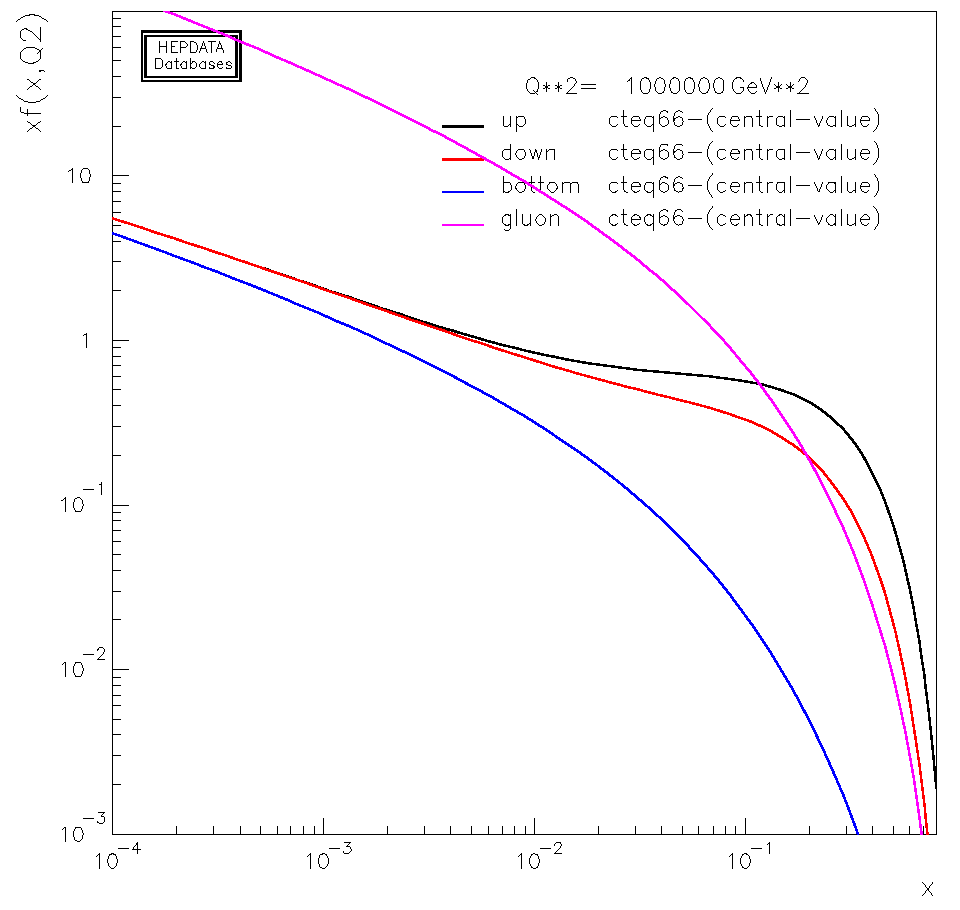
\includegraphics[width=0.45\textwidth]{\chfive/CTEQ6-pdf-set.pdf}
\caption{CTEQ6.6 central value parton distribution functions at the typical mass scale of a new diboson resonance ($Q^2 = (1000\GeV)^2$) for up, down and bottom quarks, and gluons in the proton in double-logarithmic scale.}
\label{fig:pdfs}
\end{figure}

An accurate description of the process must take into account radiative corrections to the tree-level or LO description of the process of interest.
%Indeed, a collision implies accelerated colour (and often electromagnetic) charges, and thereby bremsstrahlung can occur.
%Emissions that can be associated with the two incoming colliding partons are called Initial-State Radiation (ISR).
%Emissions that can be associated with outgoing partons are instead called Final-State Radiation (FSR).%, and can be approximated be time-like parton showers.
In particular, one has to include the effects of real and virtual higher-order corrections in perturbation theory.
This is achieved by computing the matrix element between the initial and final states as the sum of contributions with increasing powers of $\alpha_S$.
For instance, the LO contribution to the W boson production process can be calculated from the diagram in Fig.~\ref{fig:wjetsFD_LO}.
The diagrams contributing at NLO to this process and corresponding to the real and virtual radiative corrections at the first order are shown in Fig.~\ref{fig:wjetsFD_NLO}.\\

\begin{figure}[!htb]
\centering
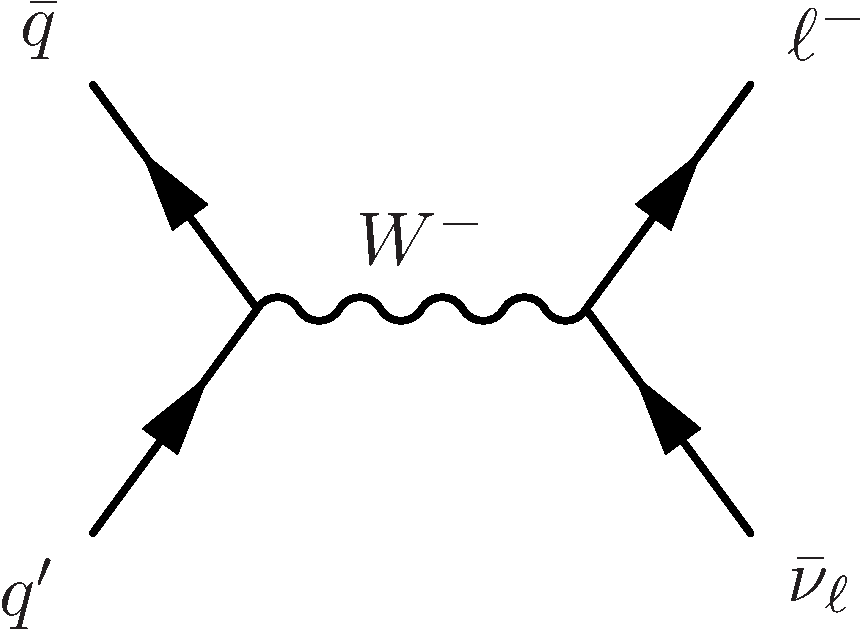
\includegraphics[width=0.3\textwidth]{\chfive/WplusJets_LO.pdf}
\caption{(top) Feynman diagram contributing to the W boson production at leading order. The charge conjugate production mode is implied. Only the leptonic decay of the W boson is considered.}
\label{fig:wjetsFD_LO}
\end{figure}

\begin{figure}[!htb]
\centering
\subfigure[]{\label{fig:wjetsFD_NLO_a}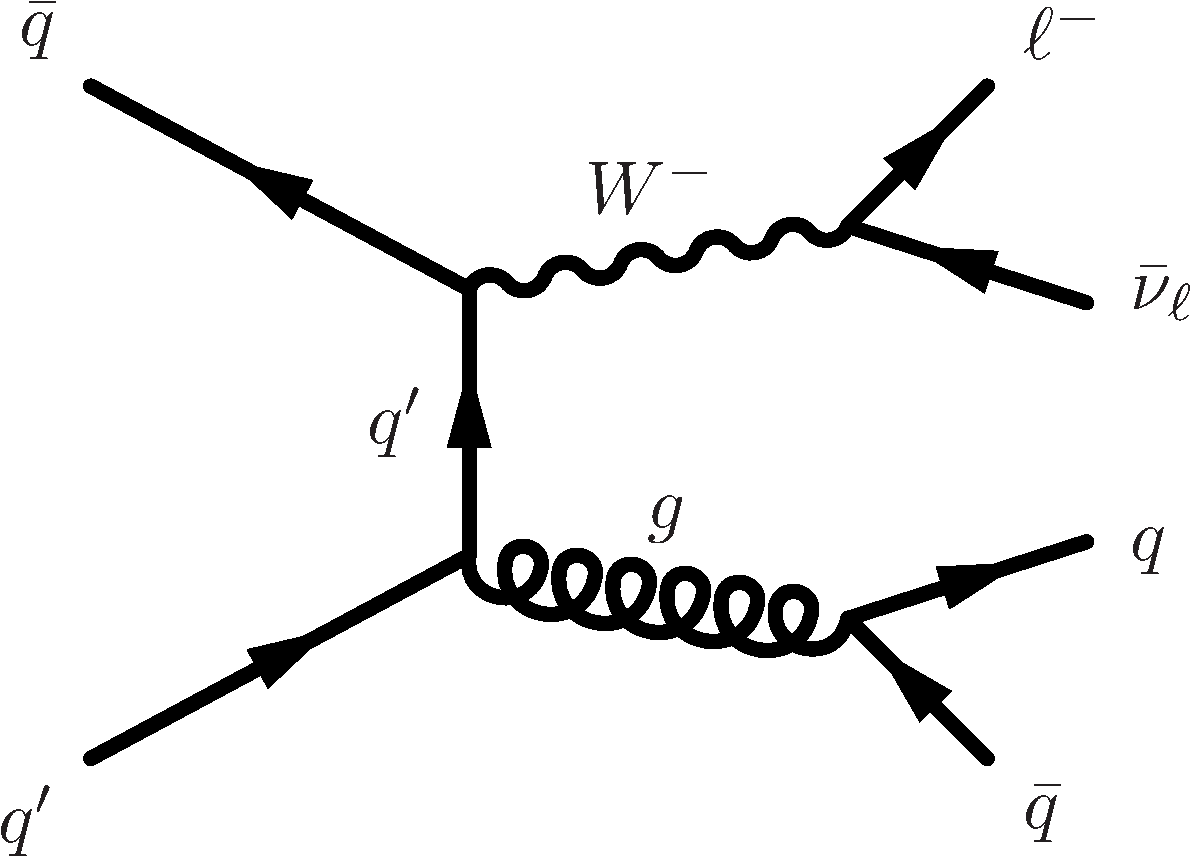
\includegraphics[width=0.3\textwidth]{\chfive/WplusJets_NLO_1.pdf}}
\subfigure[]{\label{fig:wjetsFD_NLO_b}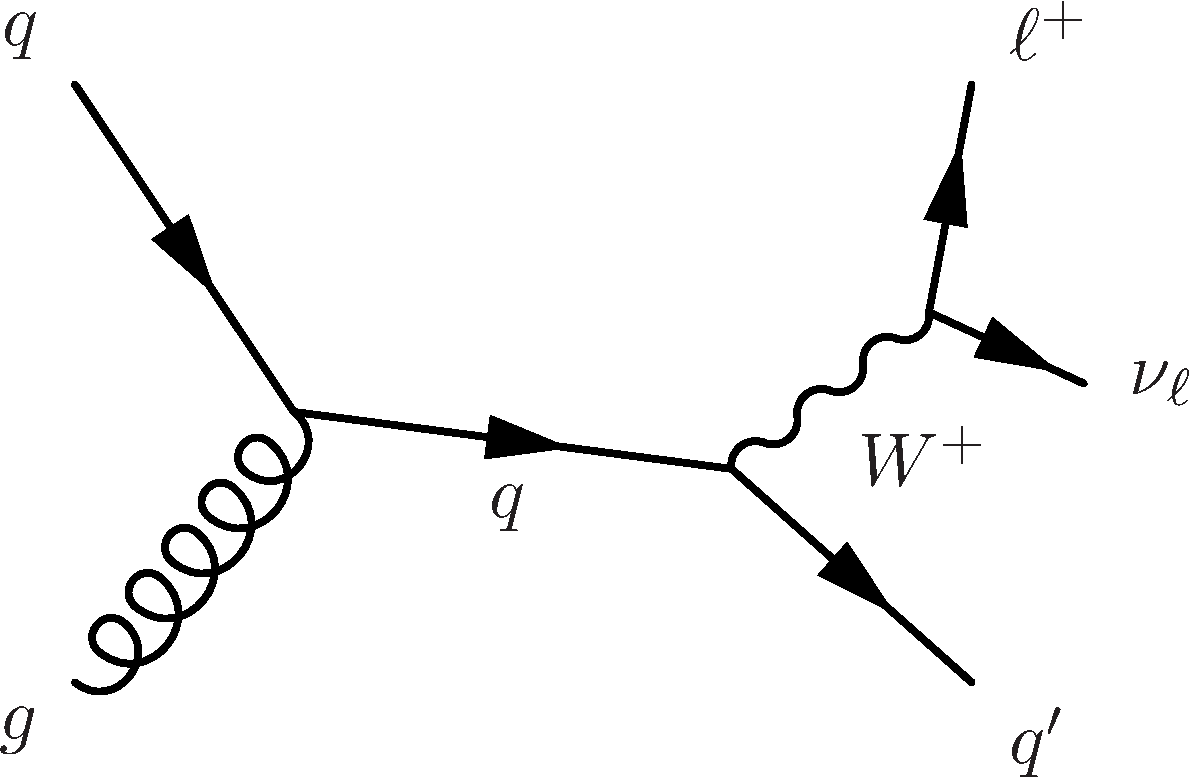
\includegraphics[width=0.3\textwidth]{\chfive/WplusJets_NLO_2.pdf}}\\
\subfigure[]{\label{fig:wjetsFD_NLO_c}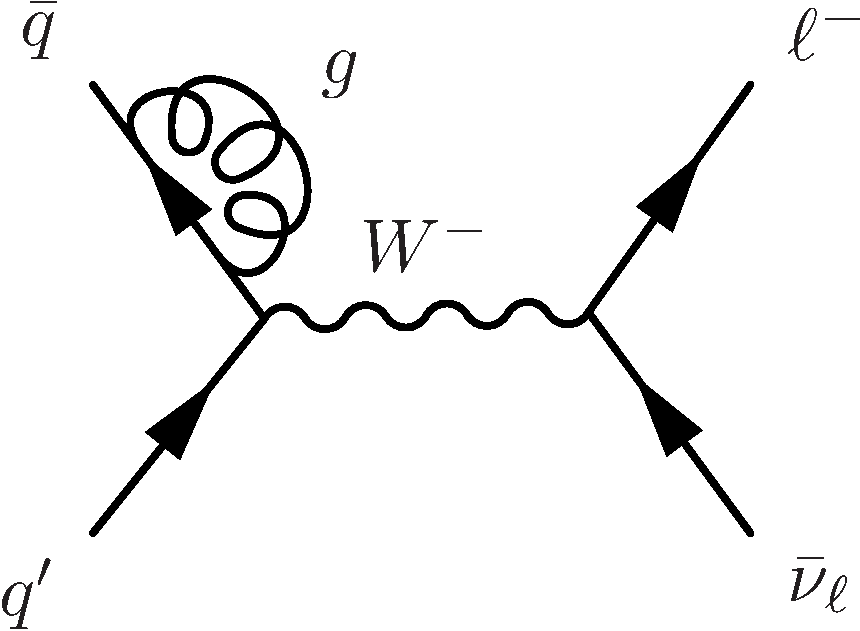
\includegraphics[width=0.3\textwidth]{\chfive/WplusJets_NLO_3.pdf}}
\subfigure[]{\label{fig:wjetsFD_NLO_d}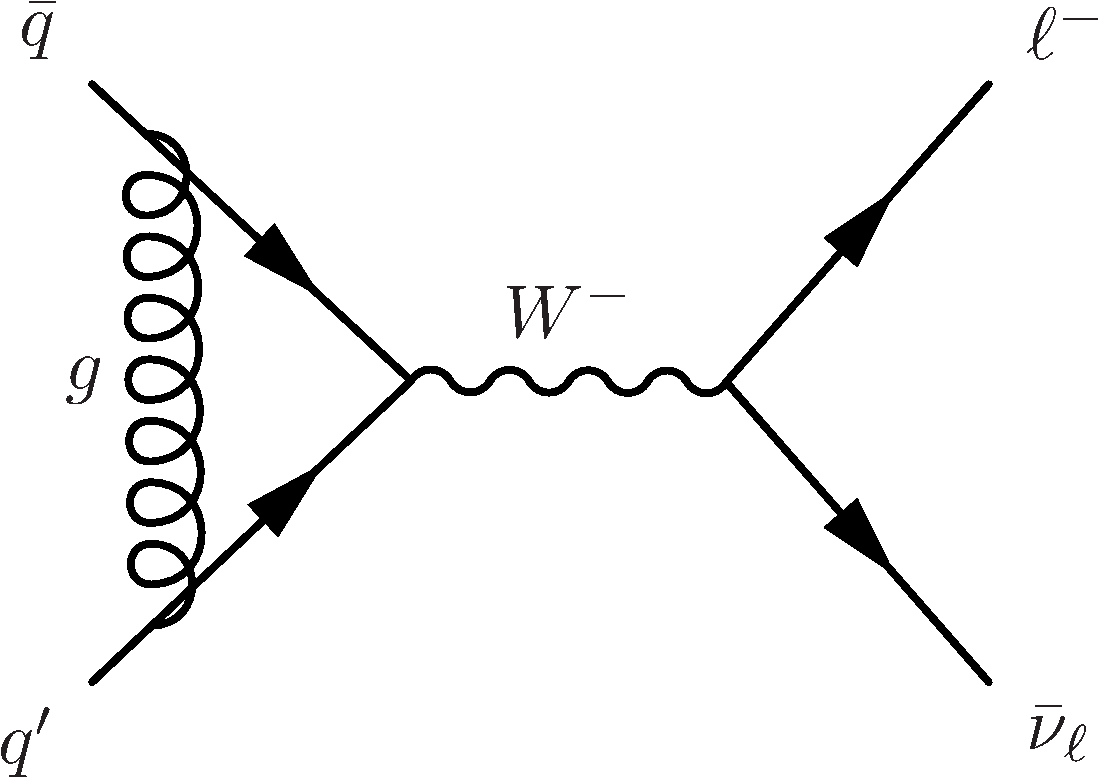
\includegraphics[width=0.3\textwidth]{\chfive/WplusJets_NLO_4.pdf}}
\subfigure[]{\label{fig:wjetsFD_NLO_e}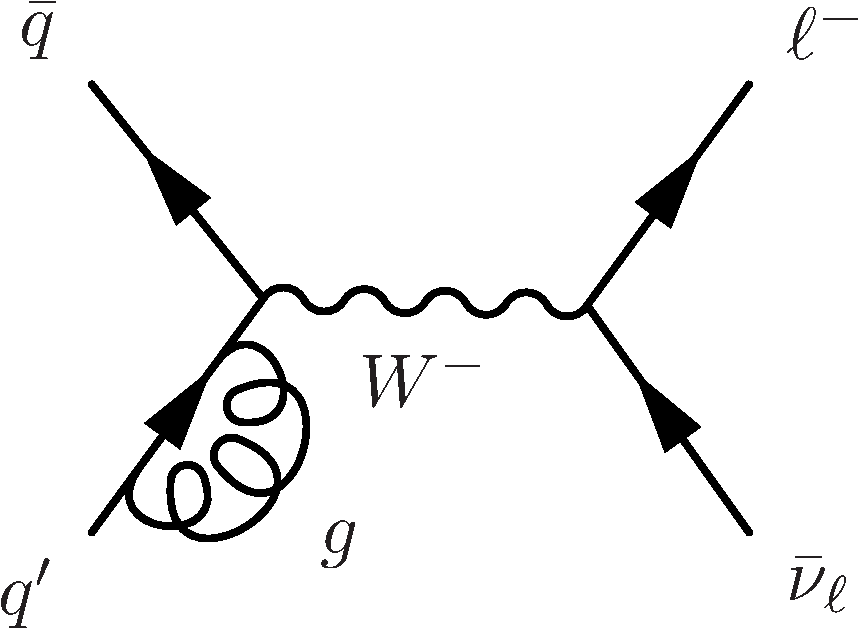
\includegraphics[width=0.3\textwidth]{\chfive/WplusJets_NLO_5.pdf}}
\caption{Feynman diagrams contributing at next-to-leading order to the W boson production and corresponding to the first order real (top) and virtual (bottom) radiative corrections.
The charge conjugate production modes are implied. Only the leptonic decay of the W boson is considered.}
\label{fig:wjetsFD_NLO}
\end{figure}

Perturbative calculations in QCD are limited to processes in which the coupling constant $\alpha_S$ is small, and by the complexity of higher order calculations preventing their evaluation.
Consequently, the current generators are only able to treat a limited number of partons in the final state. 
Parton showering algorithms extend the fixed order calculations beyond these limiting factors by calculating emissions of additional partons from the in- and outgoing partons of the main interaction.
This approach in principle takes into account emissions of an unlimited number of partons, but, as opposed to full higher order calculations, does not take into account loop diagrams.
Parton showering algorithms start from the hard process allowing the partons to split (or branch) into pairs of other partons.
These again may also branch and so on, so that an event then consists of a large number of elementary particles, including quarks and gluons.
The cascade of splittings is stopped once the energy scale reaches values where the coupling constant $\alpha_S$ becomes large.

At this stage, quarks and gluons, which carry colour, cannot be considered as free anymore and recombine to form neutral hadrons, through the so called \textit{hadronization} process.
The formation of color-neutral hadrons from the colored partons is treated in phenomenological non-perturbative models.
Eventually, many short-lived resonances will be present after hadronization which are then decayed.

The showering and hadronization programs often bring along the possibility to add underlying events. The underlying event arises from the colored remains of the protons that did not take part in the hard collisions, the so-called beam remnants.
They are usually included in the hadronization process, because they might be colour-connected to the hard subprocess. The produced hadrons will however carry a very small transverse momentum and will be very forward.
The probability for colour reconnection to take place between two partons can also be adjusted based on experimental data. %---> tuning!
It is also possible that more than one parton interact with the other proton. This phenomenon, called multiple parton interaction, and it is usually added to the description of the process.\\
%Furthermore, at the LHC there is the possibility of multiple parton interactions from the beam protons that are also added.

As last step the pileup is also accounted for.
Additional simulated minimum-bias interactions are added to the generated events to match the additional particle production due to pileup.
%The MC samples are overlaid with simulation samples reproducing the bunch train structure of the LHC beams.
%This is particularly important to take into account out-of-time pileup, i.e. additional collisions taking place before or after the actual bunch crossing of interest.
The exact number of average collisions per bunch crossing in the data is estimated by multiplying the instantaneous luminosity, continuously monitored, by the total inelastic cross section.
One can then reconstruct the distribution of the number of pileup interactions in the data for the complete data taking.
The corresponding distributions for the 2012 and 2015 data are shown in Figs.~\ref{fig:pu_mc_data_a} and~\ref{fig:pu_mc_data_c}, respectively, together with the corresponding simulated pileup scenarios.
Simulated events are then reweighted such that they match the data distribution. The description of the pileup by the simulation can be verified by counting the number of reconstructed vertices in the event as illustrated in Figs.~\ref{fig:pu_mc_data_b} and~\ref{fig:pu_mc_data_d}.\\

\begin{figure}[!htb]
\centering
\subfigure[]{\label{fig:pu_mc_data_a}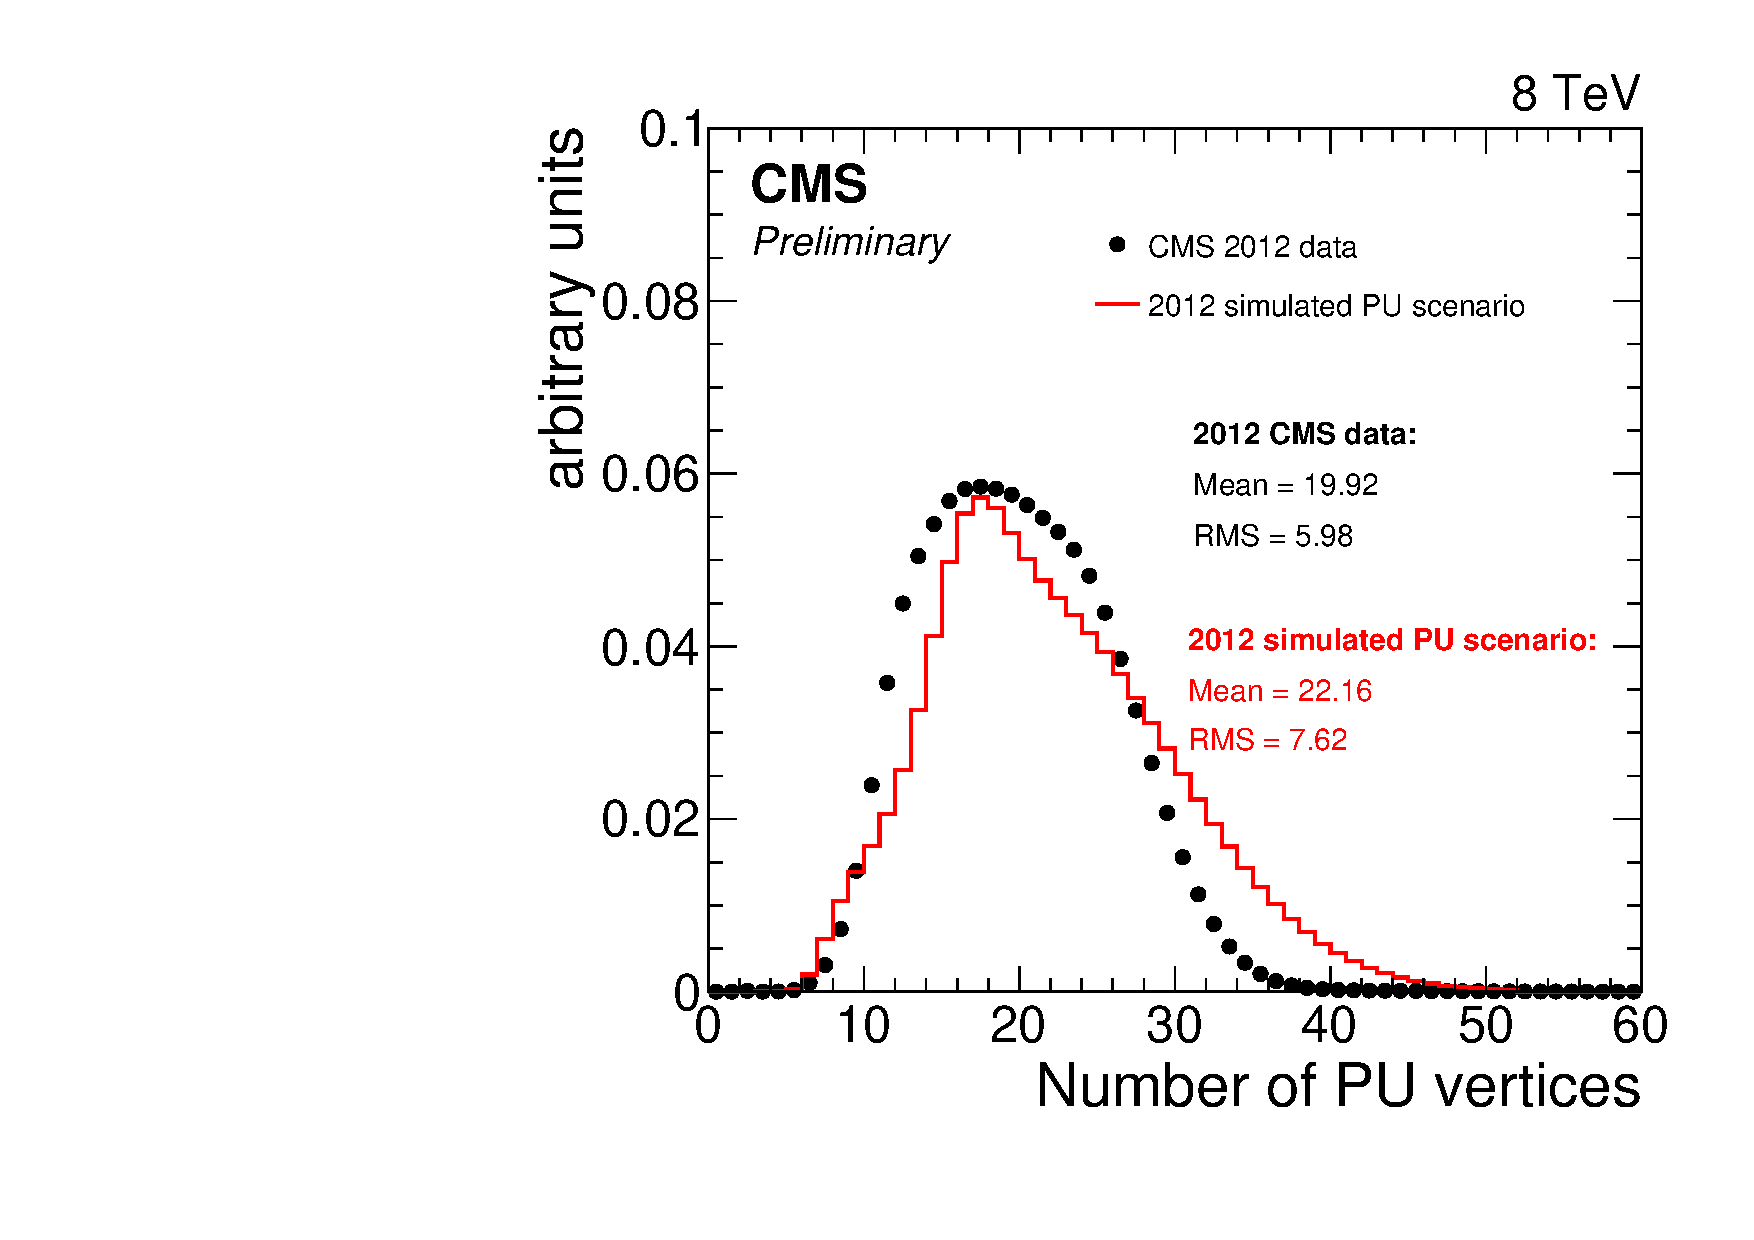
\includegraphics[width=0.47\textwidth]{\chfive/PU-data-mc-8TeV.pdf}}
\subfigure[]{\label{fig:pu_mc_data_b}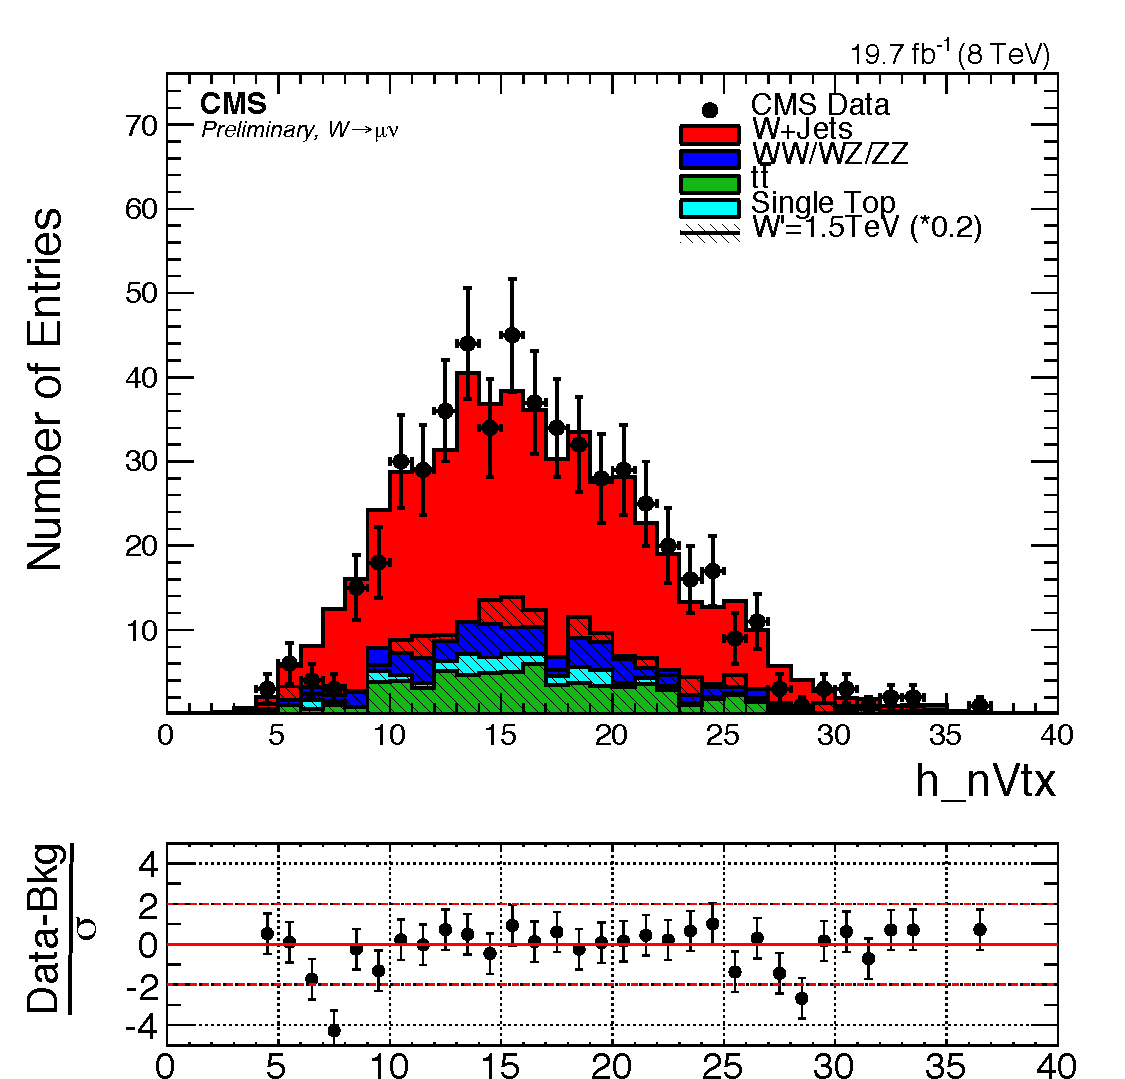
\includegraphics[width=0.44\textwidth]{\chfive/can_h_nVtx.pdf}}\\
\subfigure[]{\label{fig:pu_mc_data_c}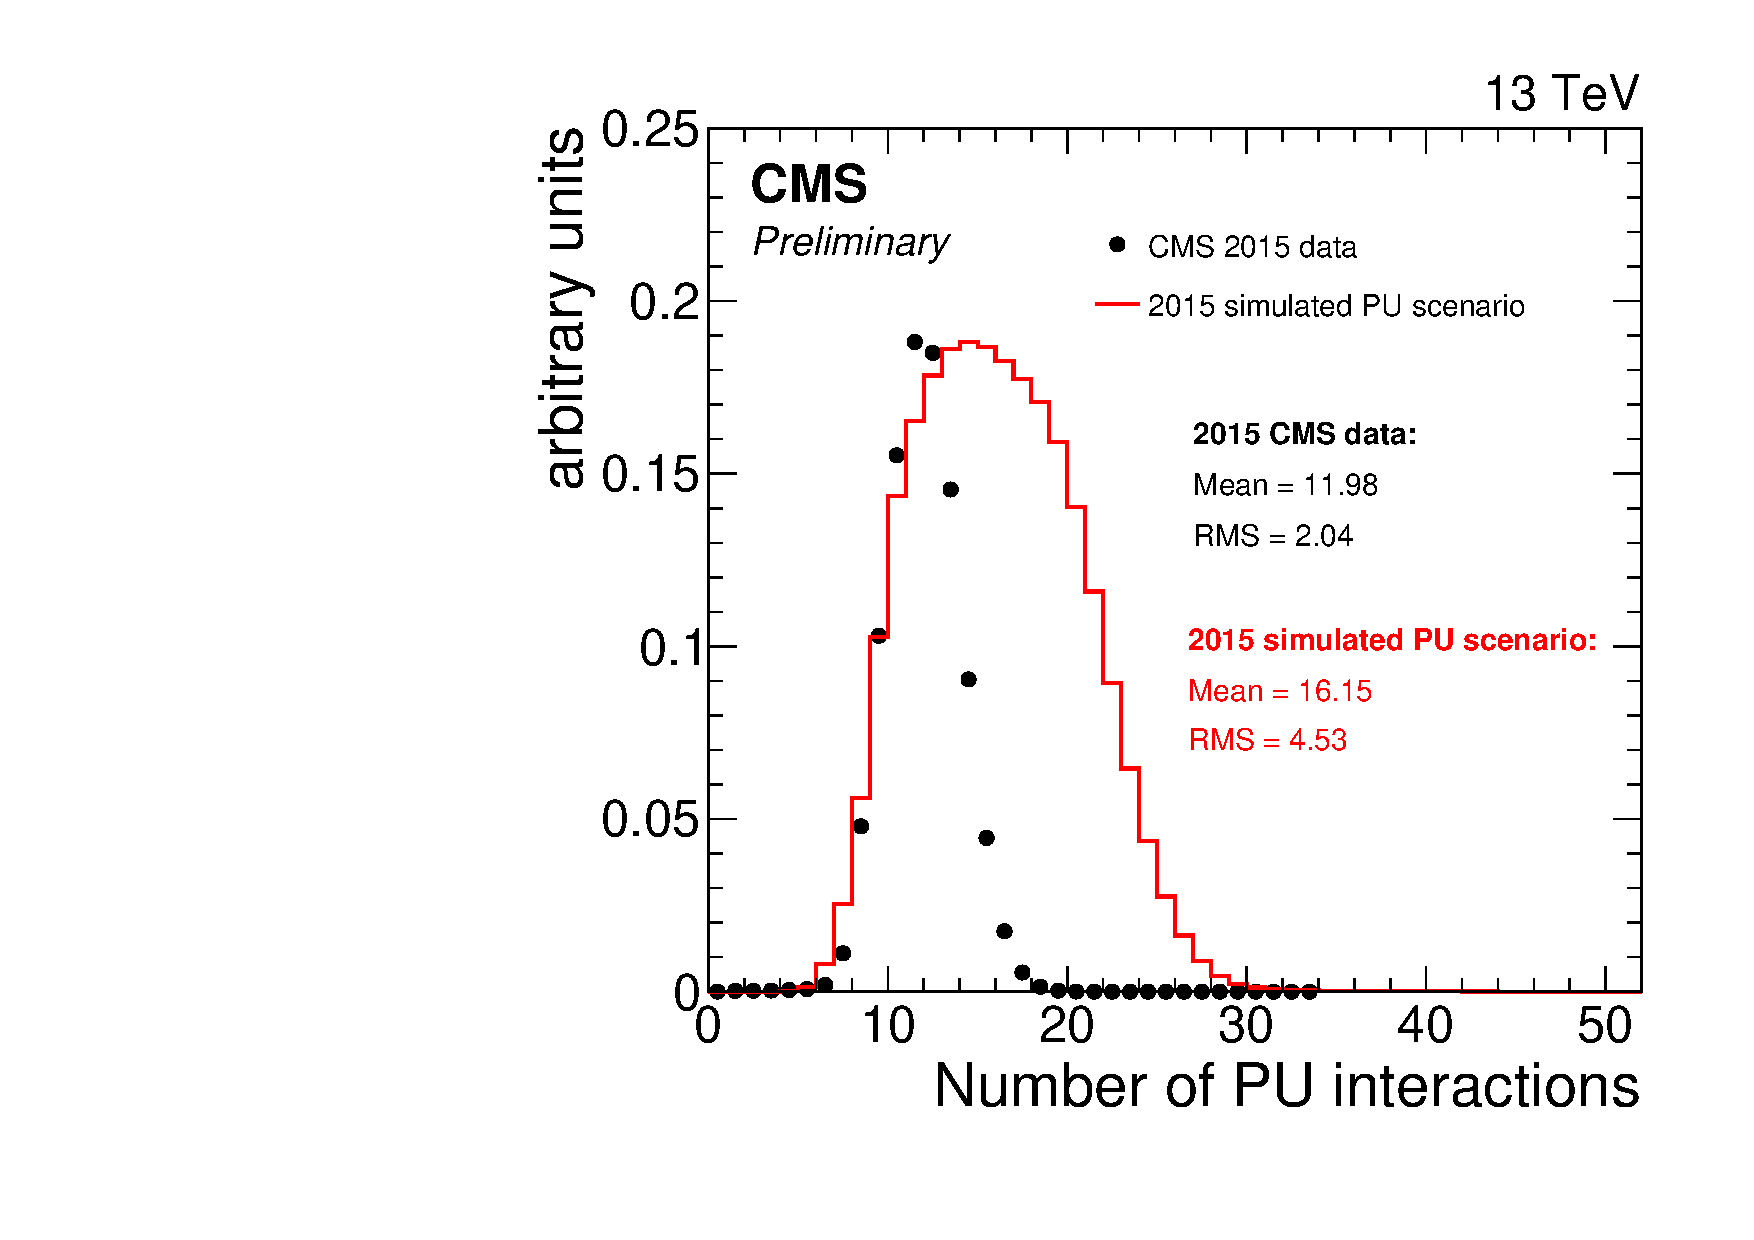
\includegraphics[width=0.47\textwidth]{\chfive/PU-data-mc-13TeV.pdf}}
\subfigure[]{\label{fig:pu_mc_data_d}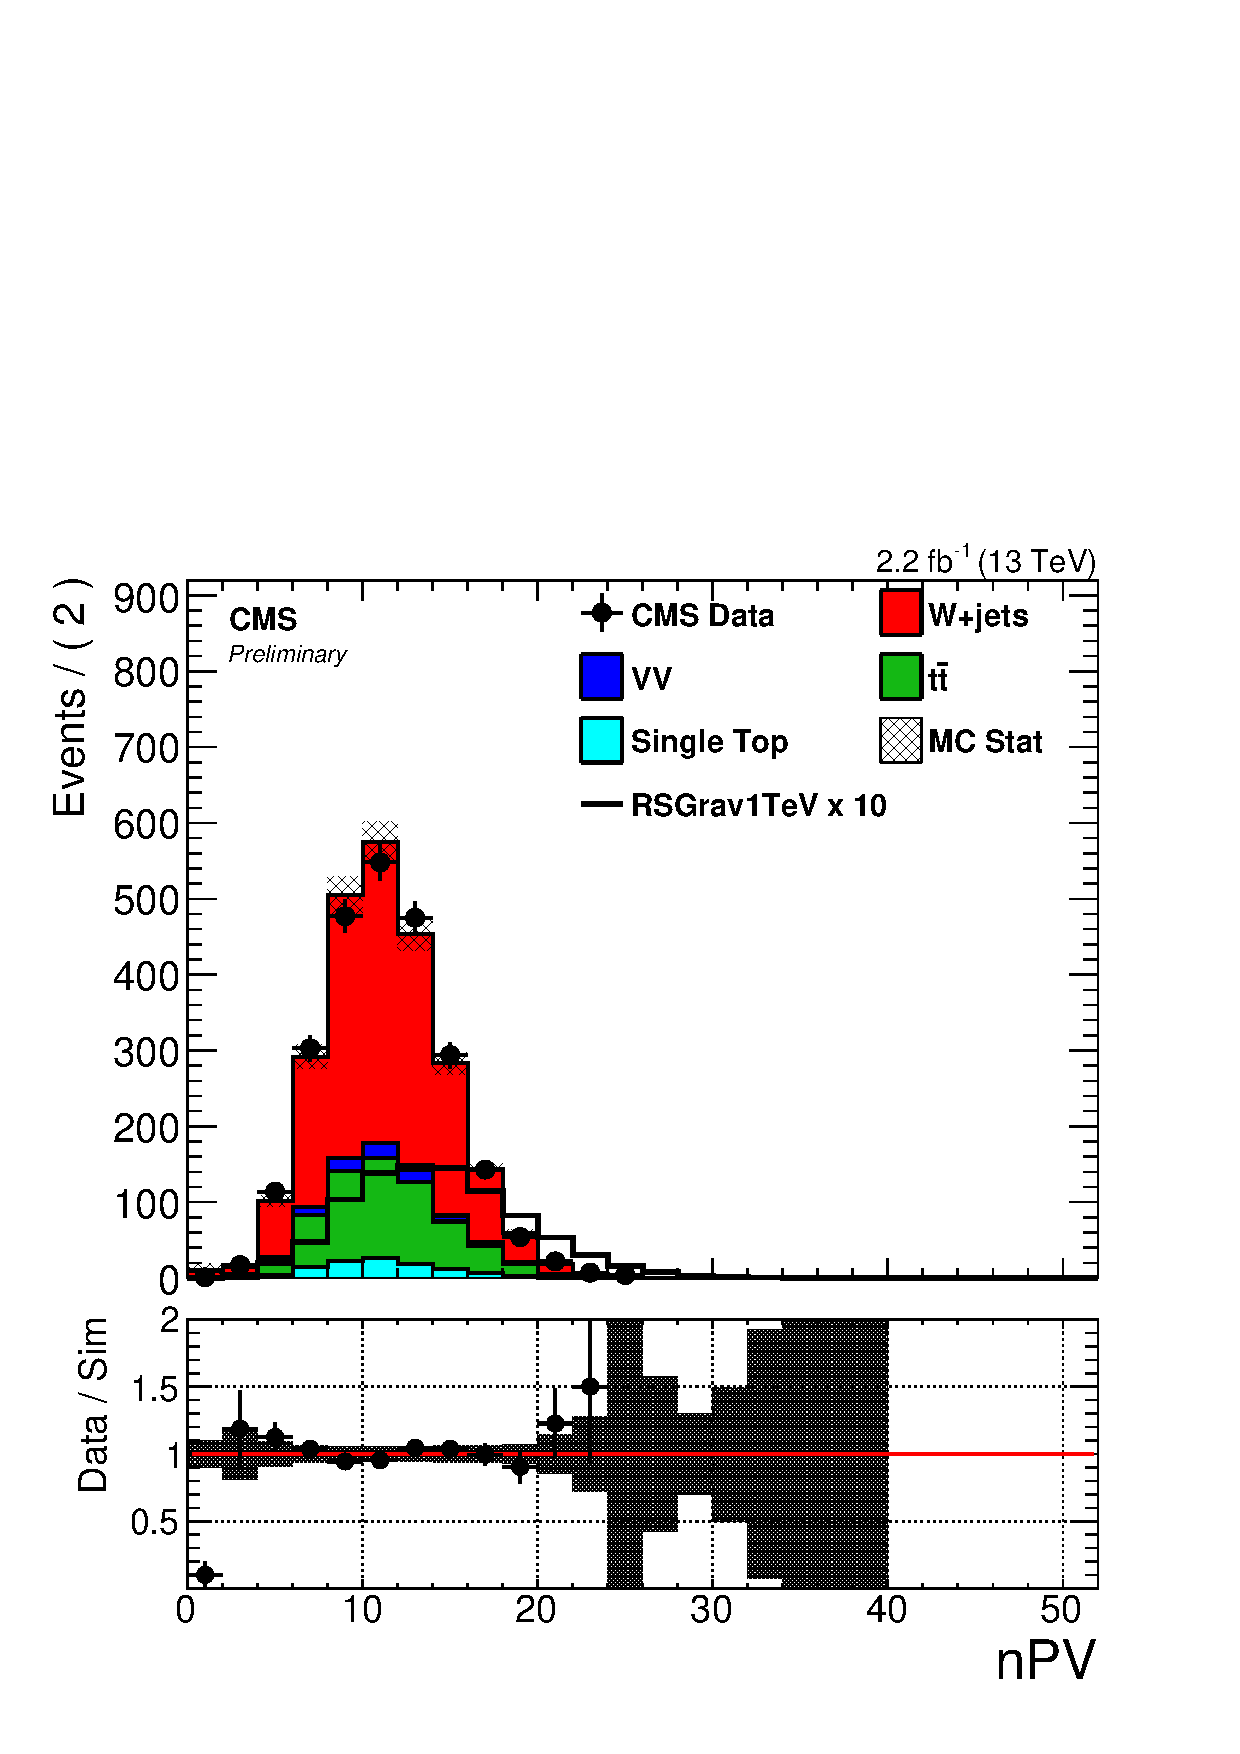
\includegraphics[width=0.44\textwidth]{\chfive/nPV_0.pdf}}
\caption{Distributions of the estimated average number of pileup collisions in the full data set of pp collisions recorded at $\sqrt{s} = 8\TeV$ in 2012 (a) and at $\sqrt{s} = 13\TeV$ (c), together with the corresponding simulated pileup scenarios. Also shown are the distributions of the number of reconstructed primary vertices in 8\TeV (b) and 13\TeV (d) data (black dots) and in various simulated samples after pileup reweighting, for lepton+jet events.}
\label{fig:pu_mc_data}
\end{figure}

Currently, NLO available calculations included in MC event generators cover a wide range of physics processes, starting with two particles annihilation to a maximum of five final state objects.
%Various generators are available to generate events according to a given hard process~\cite{Dobbs:2004qw}.
%Although all the orders of the perturbative development should be considered, most of the event generators only include the leading contribution to the matrix element.
A popular generator is \PYTHIA{}~\cite{Sjostrand:2007gs,Sjostrand:2006za}, a general purpose program which, in addition to the hard process, also takes care of the parton showering, the hadronization, and the description of the underlying event.
For the matrix element calculation, \PYTHIA{} only considers the leading order hard subprocess (diagram in Fig.~\ref{fig:wjetsFD_LO} for the W production case), and higher
order effects are added by ``evolving'' the event using the parton shower.
%The radiative corrections are not explicitely calculated but rather treated in the parton showering.
%As will be discussed in the next section, the parton showering is well suited to treat low $Q^2$ radiation.
%It however fails to accurately describe hard radiations. The consequence is that the performances of \PYTHIA{} to describe events including many hard jets in the final state are limited.
A more accurate approach is followed by \MADGRAPH{}~\cite{Alwall:2011uj} where the hard real radiative
corrections are included in the matrix element (Fig.~\ref{fig:wjetsFD_NLO}). %Diagrams with up to 5 extra partons are included.
This generator is well suited to study processes such as W or Z produced in association with hard jets.
Since it does not completely simulate the events, it needs an additional program, typically \PYTHIA{}, to perform the parton shower after the calculation of the matrix element.
It has to be noted that matrix element generators as well as shower and hadronization generators are usually treated independently: the matrix element generators compute the hard process at fixed-order and the parton shower processes the soft and collinear emissions. However, this fails to correctly represent higher order processes in which an additional parton is emitted at the hard scale because parts of this process overlap with the soft one. Combining an NLO matrix element program with a parton shower program therefore leads to double-counting of events. The NLO matrix element generators, such as \POWHEG{}~\cite{Frixione:2007vw} and \MCATNLO{}~\cite{Frixione:2003ei}, take special care of the merging of soft and collinear emissions and hard ones.
%They allow to calculate any amplitudes at NLO accuracy, and include the matching to the parton shower to produce events ready for the hadronization.
%The automatic event generator at next to leading order, \MCATNLO{}~\cite{Frixione:2003ei}, allows to calculate any amplitudes at NLO accuracy, and includes the matching to the parton shower to produce events ready for the hadronization.
%The \POWHEG{}~\cite{Frixione:2007vw} generator is another approach to calculate NLO matrix elements matched with the parton shower.
%As for \MADGRAPH{}, after the generation, the \POWHEG{} output needs to be interfaced to a chosen showering program, for example \PYTHIA{}.
%Finally, the \POWHEG{}~\cite{Frixione:2007vw} generator is a complete next to leading order (NLO) generator that considers both real and virtual corrections at the leading order.
%It is therefore limited to the radiation of one hard extra parton after what it must rely on the parton showering description.
%The use of the full NLO nevertheless provides in general an accurate estimate of the inclusive cross section. 
%In addition to event generators, there also exist cross section integrators which can be used to compute cross sections as a function of a variable of interest.
%An example is the FEWZ code [97] which allows one to make calculation at the NNLO level for exclusive production of a W or Z boson.
%cle mens: about generators
%Since the first parton radiation is already described, the interface between \POWHEG{} and the parton showering requires some special treatment.

%%%%
\subsection{CMS detector simulation}\label{subsec:fullSim}
%%%%

For a detailed understanding on how interactions in pp collisions at the LHC are observed by the CMS detector, a dedicated simulation of the whole detector is needed.
Both the propagation of particles through the detector material as well as the response of the active detector components and their digital output need to be simulated.
The input to the detector simulation are collections of particles produced by MC event generators. The output is the digital signal from all detector components in the same format that is used for real data.

The CMS simulation is based on the \GEANTfour~\cite{Agostinelli:2002hh} toolkit.
The program calculates the trajectory of the various particles generated during the collision, simulates their electromagnetic and hadronic interaction with the crossed material and the signal they will produce in the various subdetectors.
The detector geometry is given as an input to the program, and to obtain a description as close as possible to the reality, any available information such as the existence of insensitive materials or dead channels and their position, is included.
The electronic readout of the hits produced by particles is simulated, taking into account resolution and detector response effects.
The same algorithms as for real data are then used to reconstruct the various physical objects (Chapter~\ref{ch:EventReconstruction})
%The software used by CMS, CMSSW, is a code mainly written in the C++ language which is constantly updated by the whole collaboration to integrate new knowledge on the detector (new tracker alignment or calorimeter calibration,...) or to improve the object reconstruction.

%%%%%%%%%%%%%%%%%%%%%%%%%%%%%%%
\section{Simulated samples}\label{sec:MCsamples}
%%%%%%%%%%%%%%%%%%%%%%%%%%%%%%%

\subsection{Simulation of signal processes}\label{subsec:signalMC}

For the 8\TeV data analysis, the signal hypothesis has been simulated at LO accuracy with a \Wpr boson produced via quark-antiquark annihilation and decaying into W and Higgs bosons
in the $\ell\Pgn\qqbar$ final state with q = b, c or g and $\ell$ = e, $\mu$ or $\tau$. Resonance masses in the range 0.8--2.5\TeV are considered in this analysis.
The events are generated at parton level using a model of a generic narrow spin-1 \Wpr resonance implemented with \MADGRAPH{}.
Showering and hadronization are performed using \PYTHIA{6} using the Z2* tune~\cite{Chatrchyan:2011id,Chatrchyan:2013gfi}.
It has been verified that the kinematic distributions obtained with the implementation of the generic model 
agree with those predicted by implementations of the LH, composite Higgs and HVT models in \MADGRAPH{}.
The resonance width differs in the three models, but in each case it is found to be negligible with respect to the experimental resolution.

The full simulation of the detector has been done privately following the standard CMS procedure described in Section~\ref{subsec:fullSim}.
This emulation has been validated comparing the private production with samples from the MC production campaign carried out centrally for the whole collaboration.

The following parameters are used to compute the cross sections: $g_\mathrm{V}$ = 3, $c_\mathrm{H} \simeq -1$, and $c_\mathrm{F} \simeq 1$
in the HVT model B (\FIXME{point to theory}) and cot2$\theta$ = 2.3, cot$\theta$ = -0.20799 in the LH model, where $\theta$ is a mixing
angle parameter that determines \Wpr couplings (\FIXME{point to theory}) such that cot2$\theta$ and cot$\theta$ can be directly related to $c_\mathrm{H}$ and $c_\mathrm{F}$.

The intrinsic width and cross section for both models are listed in Table~\ref{tab:gamma_xsec_LH_HVT} for the resonance masses considered.
The widths for the HVT model B are computed by means of Equation (2.31) in Ref.~\cite{Pappadopulo:2014qza},
while the cross sections were obtained using the online tools provided by the authors of Ref.~\cite{Pappadopulo:2014qza}. (\FIXME{point to theory})

\begin{table}[!htb]
\caption{
Intrinsic total widths ($\Gamma$) and cross sections for $\sqrt{s} = 8\TeV$ ($\sigma$) for the LH model and HVT model B for different masses of a resonance $\Wpr$ decaying to WH.
The $\PW\PH\to\ell\Pgn\bbbar$ branching fraction is not included in the calculation.
}
\label{tab:gamma_xsec_LH_HVT}
\begin{center}
\small
\begin{tabular}{c|cc|cc}
\multirow{2}{*}{{Resonance mass [TeV]}} & \multicolumn{2}{c}{{LH model}} & \multicolumn{2}{c}{{HVT model B}} \\
                 & $\Gamma$ [GeV] & $\sigma$ [pb] & $\Gamma$ [GeV] & $\sigma$ [pb] \\
\hline \hline
0.8 & 7.22 & 5.09$\times 10^{-1}$ & 24.1 & 3.37$\times 10^{-1}$ \\
0.9 & 8.12 & 3.03$\times 10^{-1}$ & 27.1 & 2.48$\times 10^{-1}$ \\
1.0 & 9.02 & 1.87$\times 10^{-1}$ & 30.1 & 1.71$\times 10^{-1}$ \\
1.1 & 9.92 & 1.18$\times 10^{-1}$ & 33.1 & 1.16$\times 10^{-1}$ \\
1.2 & 10.8 & 7.65$\times 10^{-2}$ & 36.1 & 8.05$\times 10^{-2}$ \\
1.3 & 11.7 & 5.06$\times 10^{-2}$ & 39.1 & 5.59$\times 10^{-2}$ \\
1.4 & 12.6 & 3.39$\times 10^{-2}$ & 42.2 & 3.88$\times 10^{-2}$ \\
1.5 & 13.5 & 2.29$\times 10^{-2}$ & 45.2 & 2.51$\times 10^{-2}$ \\
1.6 & 14.4 & 1.56$\times 10^{-2}$ & 48.2 & 1.87$\times 10^{-2}$ \\
1.7 & 15.3 & 1.08$\times 10^{-2}$ & 51.2 & 1.30$\times 10^{-2}$ \\
1.8 & 16.2 & 7.43$\times 10^{-3}$ & 54.2 & 9.03$\times 10^{-3}$ \\
1.9 & 17.1 & 5.17$\times 10^{-3}$ & 57.2 & 6.27$\times 10^{-3}$ \\
2.0 & 18.0 & 3.61$\times 10^{-3}$ & 60.2 & 4.25$\times 10^{-3}$ \\
2.1 & 19.0 & 2.53$\times 10^{-3}$ & 63.2 & 3.02$\times 10^{-3}$ \\
2.2 & 19.8 & 1.76$\times 10^{-3}$ & 66.2 & 2.10$\times 10^{-3}$ \\
2.3 & 20.8 & 1.24$\times 10^{-3}$ & 69.2 & 1.46$\times 10^{-3}$ \\
2.4 & 21.6 & 8.67$\times 10^{-4}$ & 72.2 & 1.01$\times 10^{-3}$ \\
2.5 & 22.6 & 6.07$\times 10^{-4}$ & 75.3 & 7.31$\times 10^{-4}$ 
\end{tabular}
\end{center}
\end{table}

Figure~\ref{fig:WHmodelsWidth} shows the ratio between the resonance's natural width and mass for a \Wpr in the LH and the HVT model B.
The width is less than 5\% for the following parameter values:
$0.95 < g_\mathrm{V} < 3.76$, $c_\mathrm{H}$ = -1, and $c_\mathrm{F}$ = 1;
$g_\mathrm{V} < 3.9$, $c_\mathrm{H}$ = -1, and $c_\mathrm{F}$ = 0;
or $g_\mathrm{V} < 7.8$, $c_\mathrm{H}$ =0.5, and $c_\mathrm{F}$ = 0.
The widths for the LH model have been computed by means of Eq. (15) in Ref.~\cite{Burdman:2002ns}, and they are less than 5\%
for values of $0.084 < |\mathrm{cot}\theta| < 1.21$. Hence, in both models the resonance's natural width can be considered to be negligible compared to the experimental resolution.\\

\begin{figure}[!htb]
\centering
\subfigure[]{\label{fig:WHmodelsWidth_a}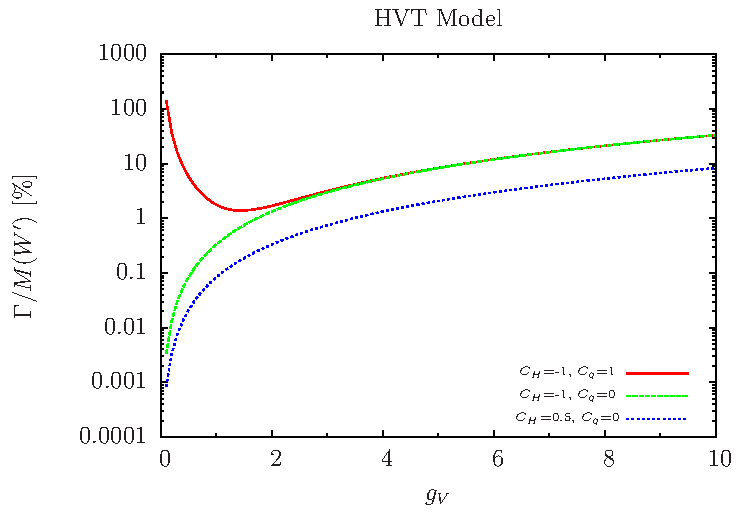
\includegraphics[width=0.45\textwidth]{\chfive/HVT.pdf}}
\subfigure[]{\label{fig:WHmodelsWidth_b}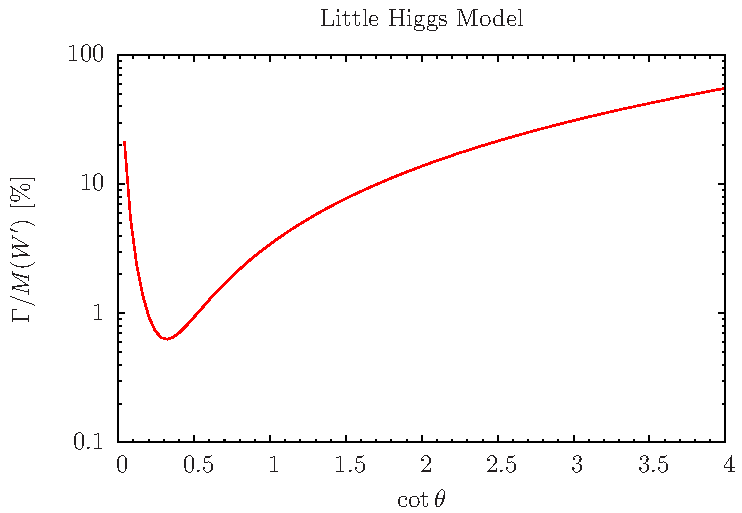
\includegraphics[width=0.45\textwidth]{\chfive/LH.pdf}}
\caption{Ratio between the resonance's natural width and mass for a \Wpr in the LH and the HVT model B.}
\label{fig:WHmodelsWidth}
\end{figure}

For the 13\TeV data analysis, the bulk graviton model and HVT models are used as benchmark signal processes.
In these models, a resonance is simulated which decays only to pairs of vector gauge bosons in the $\ell\Pgn\qqbarpr$ final state, with $\ell$ = e, $\mu$, and $\tau$.
The vector gauge bosons are produced with a longitudinal polarization in more than 99\% of the cases.
For each resonance hypothesis, masses are considered in the range 0.6 to 4.0\TeV.
Simulated signal events are generated at LO accuracy with \amcatnlo{} with a relative resonance width of 0.1\%.

The natural width of a bulk graviton as a function of the curvature parameter $\tilde{k}$ and for different mass hypotheses is shown in Fig.~\ref{fig:bulkGwidth}.
For cases in which $\tilde{k} \leq 0.5$ the relative width of the graviton resonance ($\Gamma_\mathrm{G}/\mathrm{M}_\mathrm{G}$)
is predicted to be below 1\%. Hence, it can be neglected when compared to the detector resolution over the whole explored mass range.

\begin{figure}[!htb]
\centering
\subfigure[]{\label{fig:bulkGwidth_b}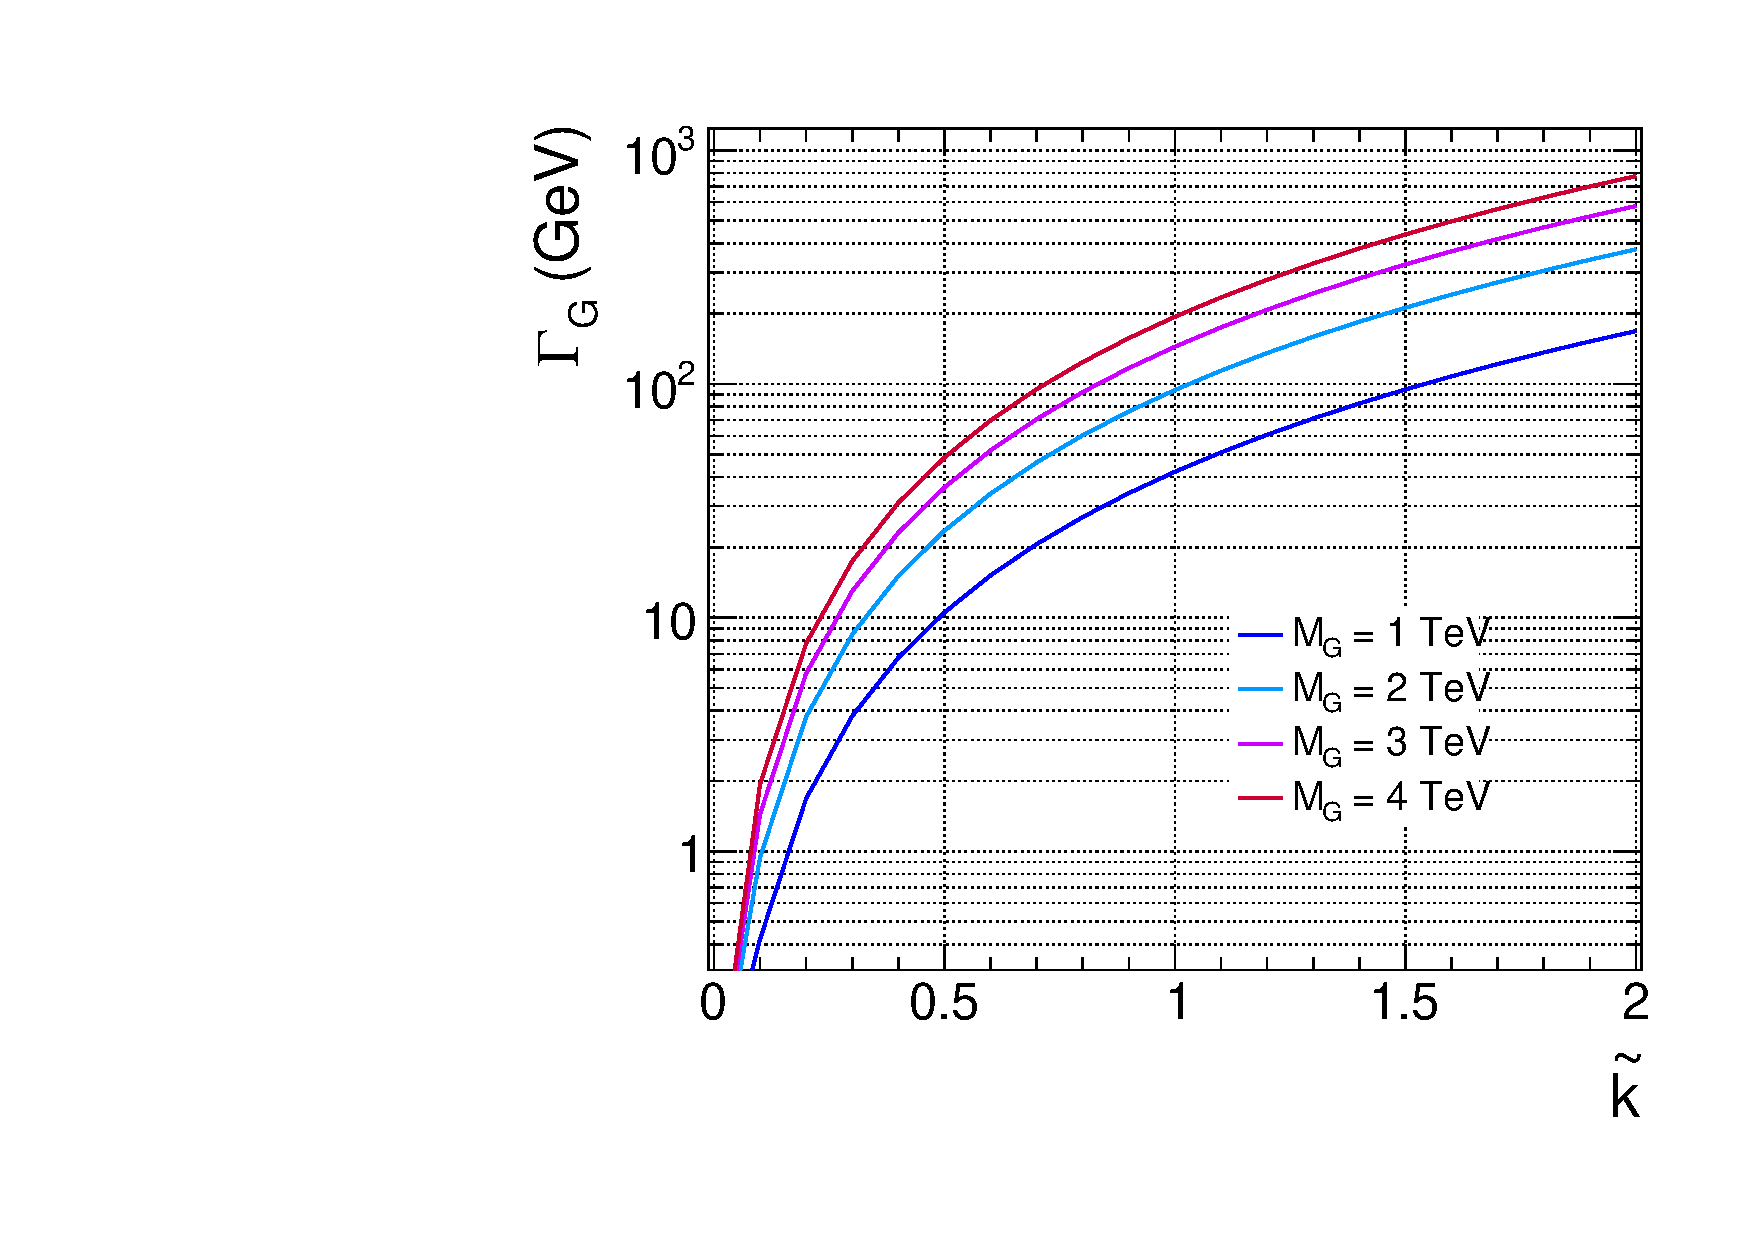
\includegraphics[width=0.45\textwidth]{\chfive/width-bulkg.pdf}}
\subfigure[]{\label{fig:bulkGwidth_a}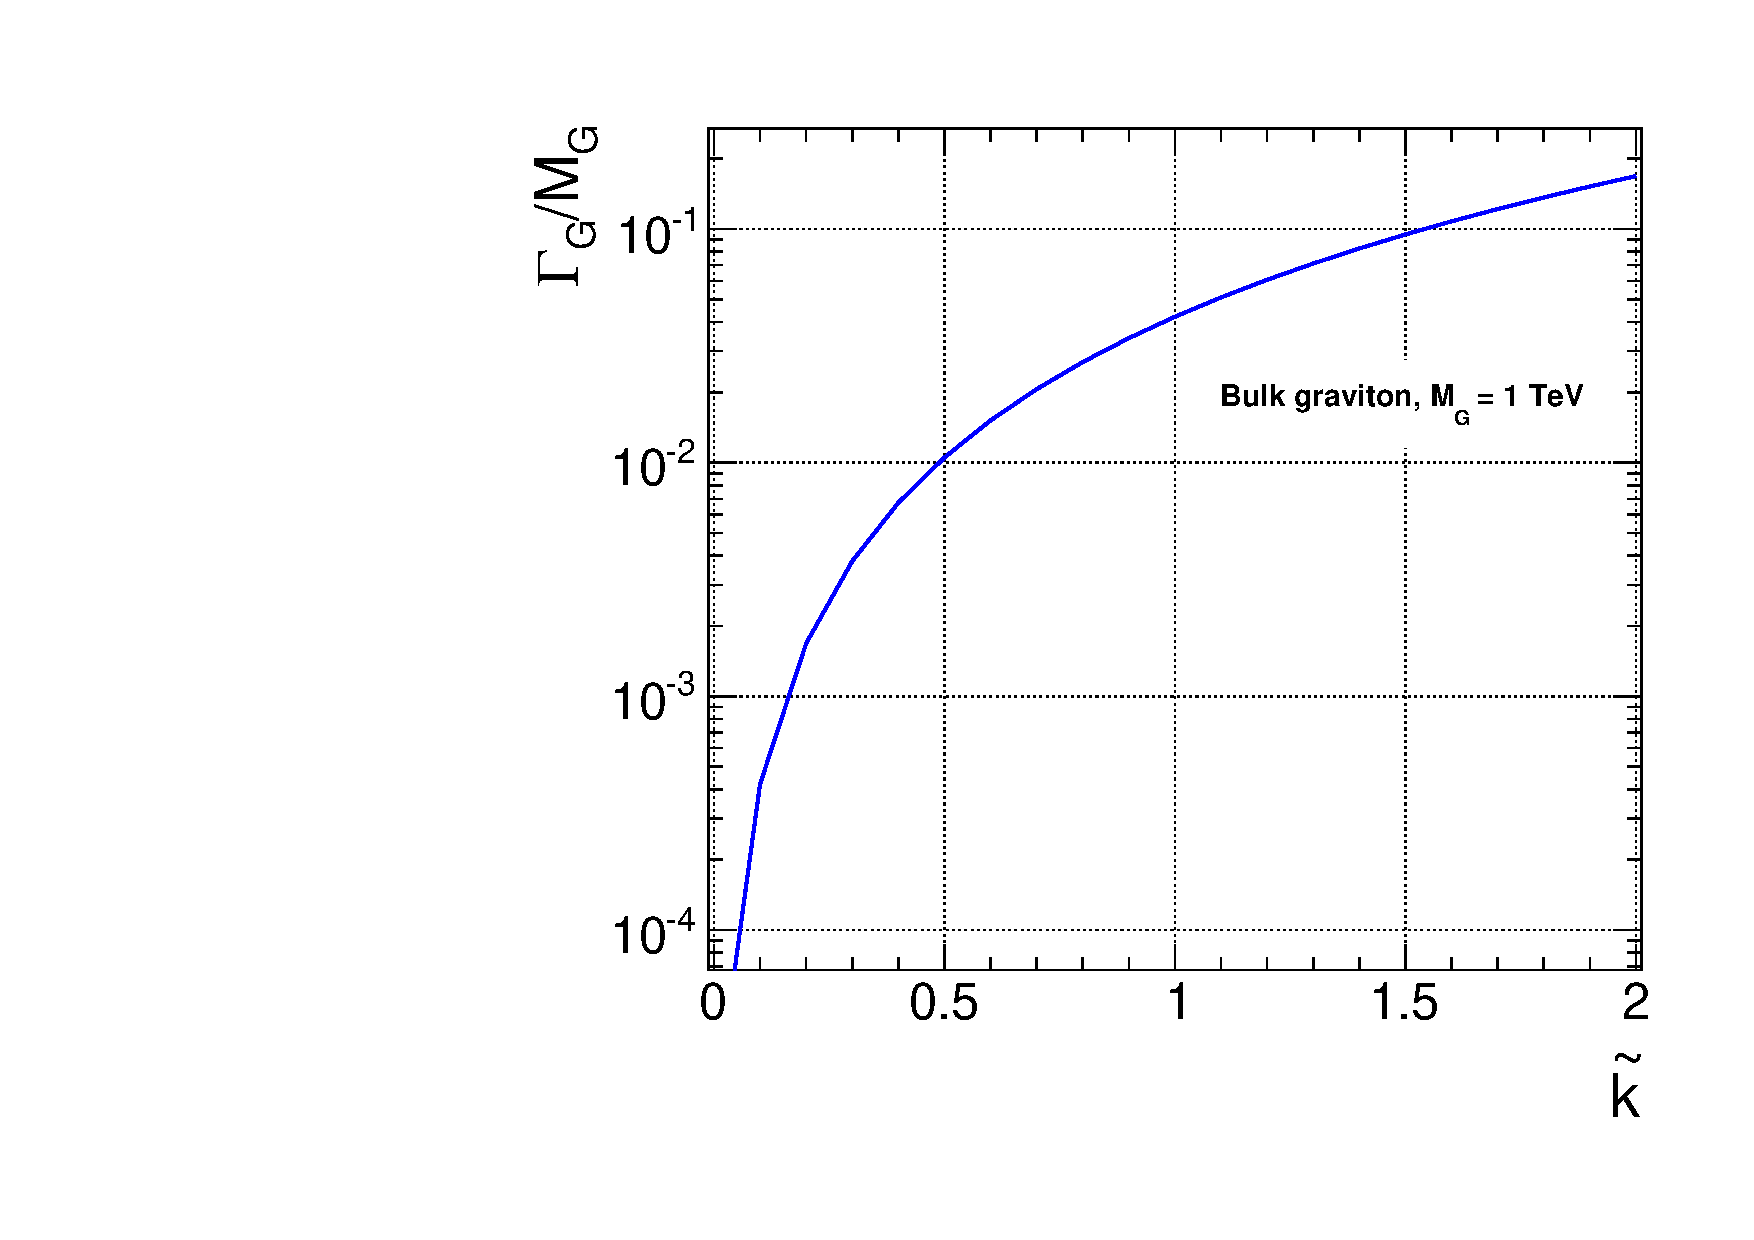
\includegraphics[width=0.45\textwidth]{\chfive/rel-width-bulkg.pdf}}
\caption{(a) Natural width of a bulk graviton as a function of the coupling constant $\tilde{k}$ and for various mass hypotheses. (b) The same dependence is expressed as relative fraction of the signal width with respect to a reference graviton mass of 1\TeV.}
\label{fig:bulkGwidth}
\end{figure}

Figure~\ref{fig:allmodelsXsec} compare the production cross sections $\sigma(\mathrm{pp}) \to X$ of the resonance for $\sqrt{s} = 8$ and 13\TeV,
for the bulk graviton with $\tilde{k} = 0.5$, and \Wpr and \Zpr in the HVT model B, as a function of the resonance mass.
Cross sections for the bulk graviton model are computed with \MADGRAPH{} with the model used for the even generation,
while values for the HVT model B are obtained using the online tools provided by the authors of Ref.~\cite{Pappadopulo:2014qza}
using the same parameters as for the 8\TeV data analysis.

For a resonance mass of 2\TeV, the production rates at for $\sqrt{s} = 13\TeV$ are expected to increase of a factor $\approx$ 17 
for a resonance produced via gluon-gluon fusion such as the graviton; a smaller factor of $\approx$ 7 is expected instead
for resonances produced via quark-antiquark annihilation such as \Wpr and \Zpr.

\begin{figure}[!htb]
\centering
\subfigure[]{\label{fig:allmodelsXsec_a}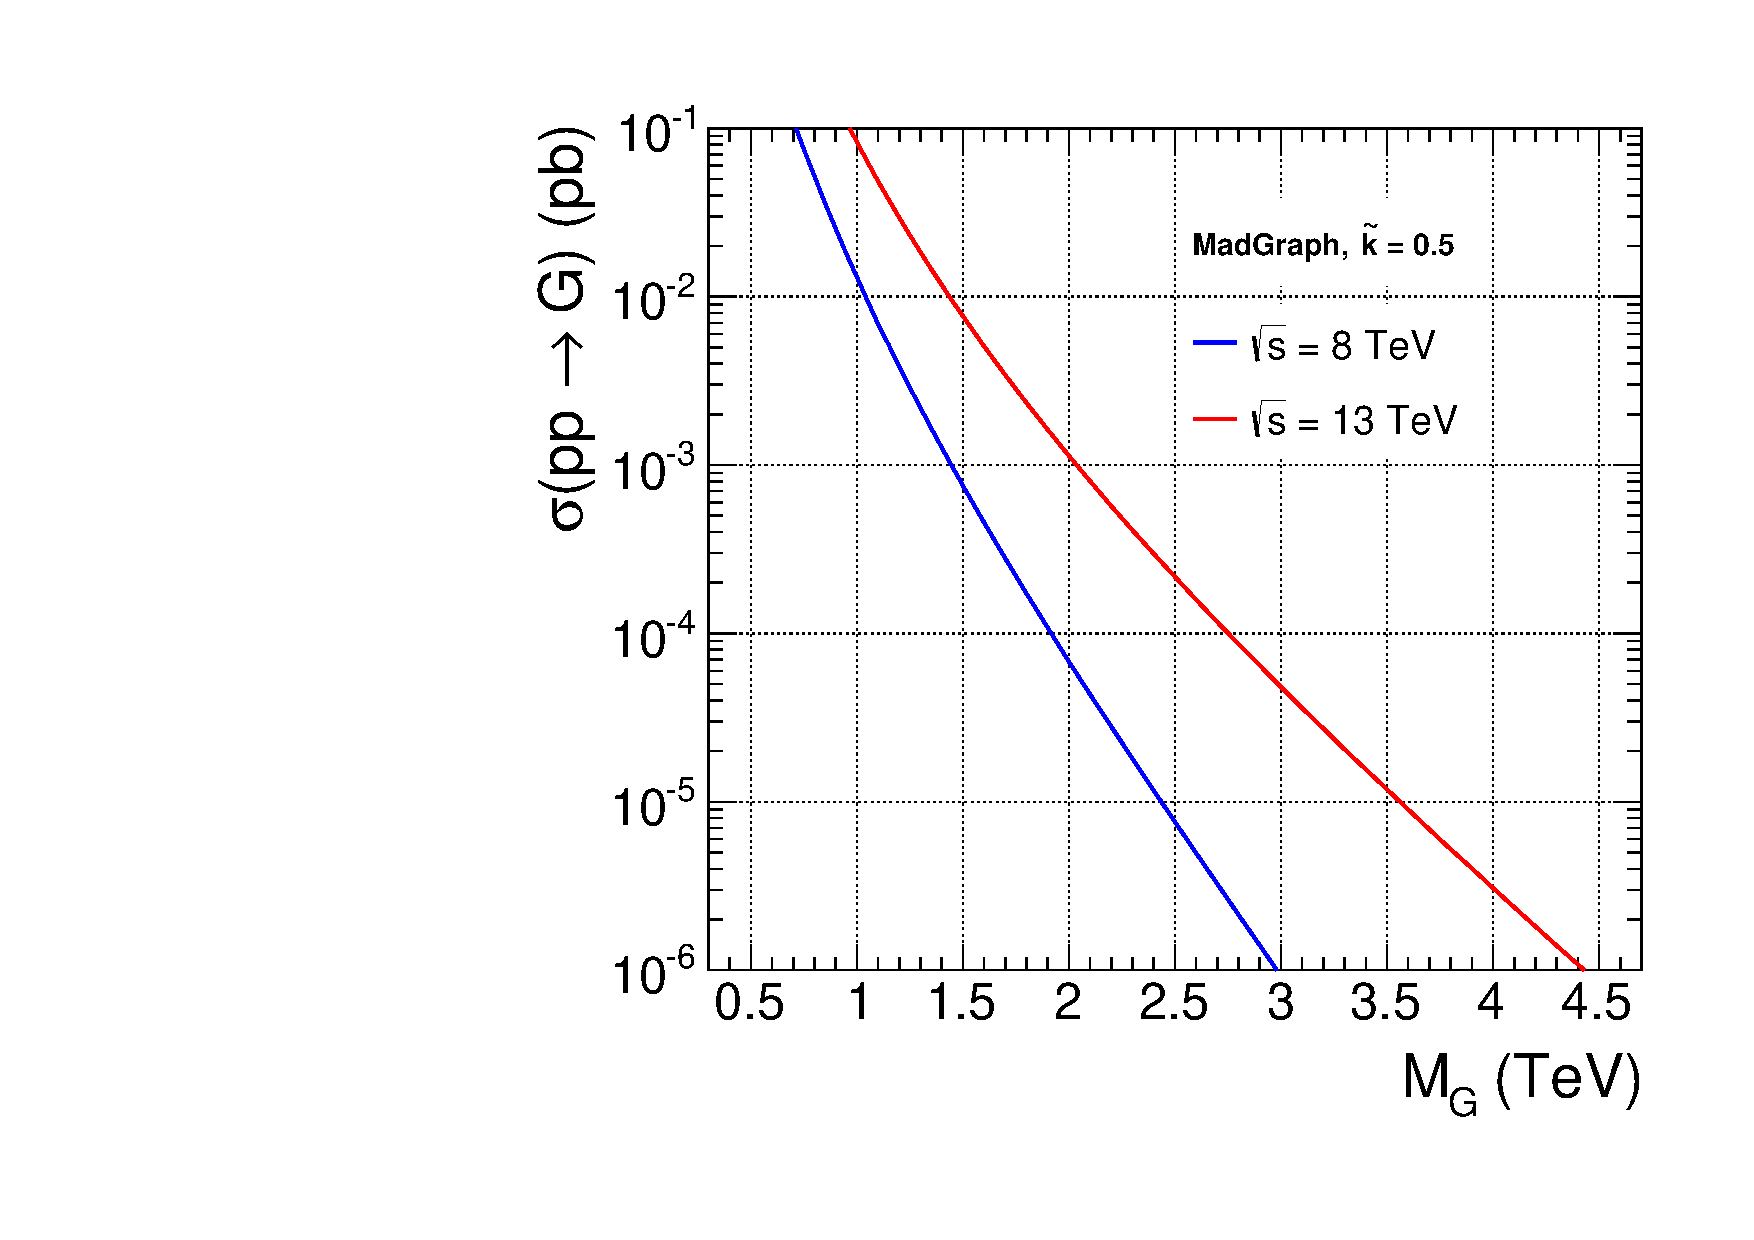
\includegraphics[width=0.45\textwidth]{\chfive/xsec-bulkg-813.pdf}}
\subfigure[]{\label{fig:allmodelsXsec_b}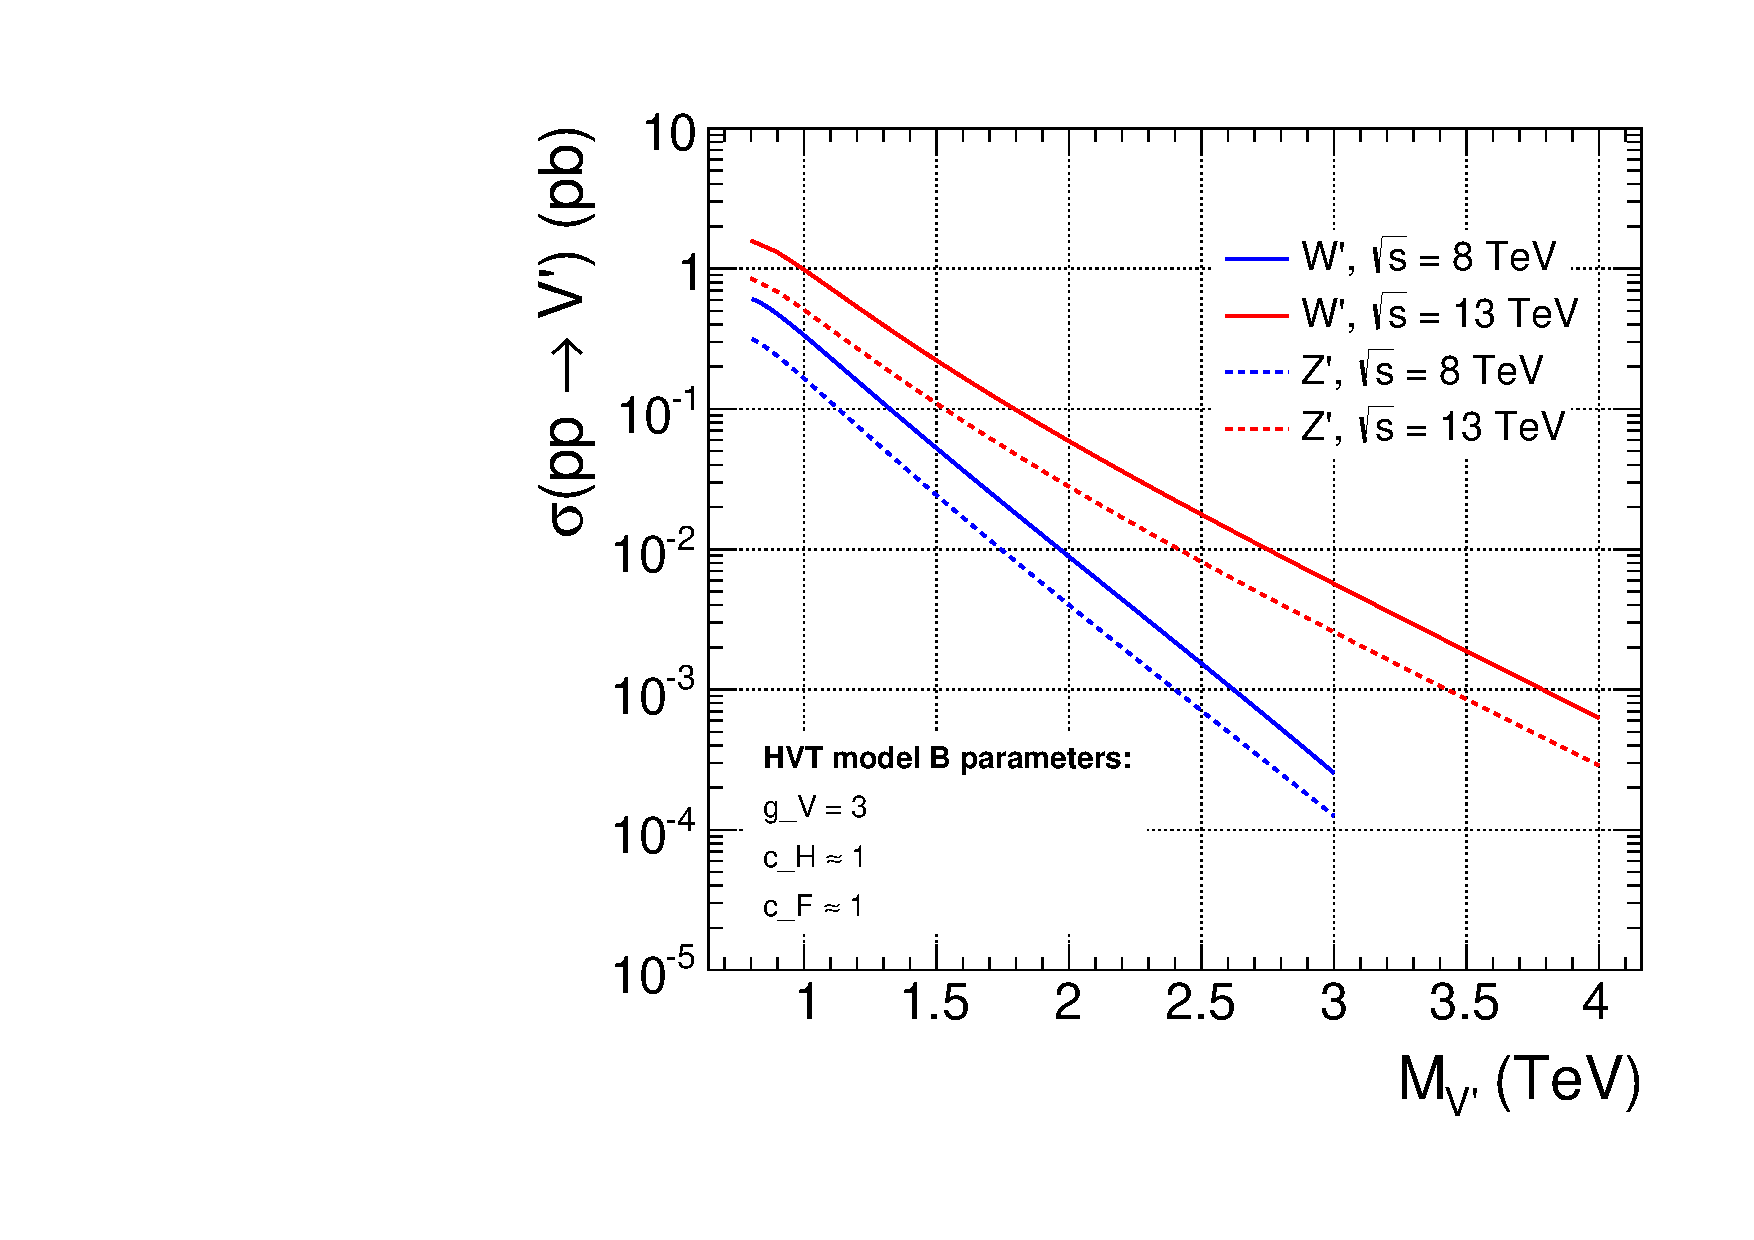
\includegraphics[width=0.45\textwidth]{\chfive/xsec-hvt-813.pdf}}\\
\subfigure[]{\label{fig:allmodelsXsec_c}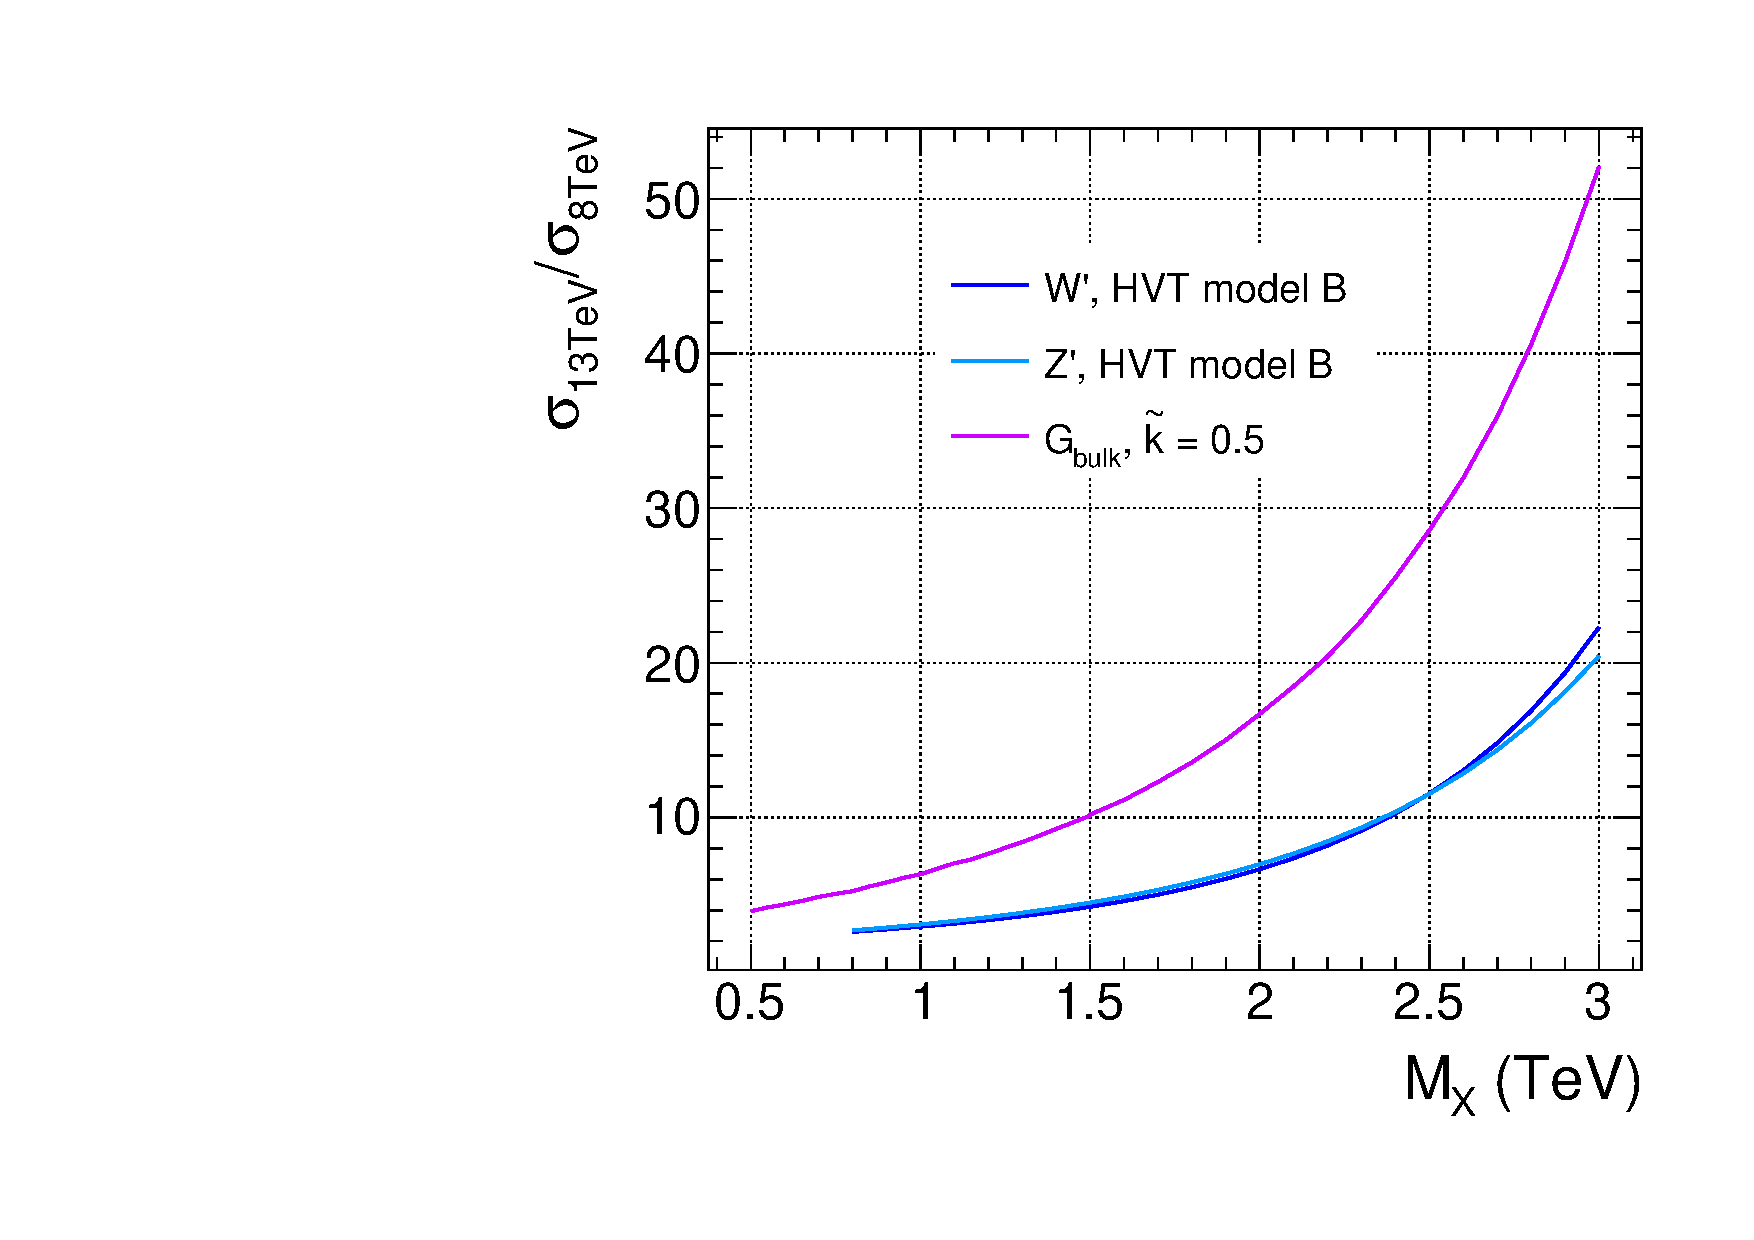
\includegraphics[width=0.45\textwidth]{\chfive/xsec-ratio-813.pdf}}
\caption{Comparison of the production cross sections of the resonance for $\sqrt{s} = 8$ and 13\TeV for the bulk graviton (a), and \Wpr and \Zpr in the HVT model B (b), as a function of the resonance mass.
(c) Ratio of the production cross sections for $\sqrt{s} = 8$ and 13\TeV for all models.}
\label{fig:allmodelsXsec}
\end{figure}

\subsection{Simulation of background processes}\label{subsec:bkgMC}

For the 8\TeV data analysis, the background is modelled using the \MADGRAPH{5} v1.3.30 event generator to simulate the production of W boson in association with jets at LO,
the \POWHEG{} 1.0 r1380 package to generate \ttbar and single top quark events at NLO accuracy, and \PYTHIA{6} v424 for SM diboson (WW, WZ, and ZZ) production at LO.
All simulated event samples are generated using the CTEQ6L1 PDF set with $\alpha_S$ also at LO, except for the \POWHEG{} \ttbar sample,
for which the CT10 NNLO PDF set is used.
All the samples are then processed further by \PYTHIA{6}, using the Z2* tune for simulation of parton showering and subsequent hadronization,
and for simulation of the underlying event. All simulated background samples are normalized to the integrated luminosity of the recorded data, using inclusive cross sections determined at NLO,
or NNLO when available, calculated with the cross section integrators \MCFM{}~\cite{Campbell:2003hd,Campbell:2011bn,Campbell:2012uf,Campbell:2004ch}
and \textsc{fewz}~\cite{Li:2012wna}, except for the \ttbar sample, for which \textsc{top++}~\cite{Czakon:2011xx} is used.
The NNLO cross section for the W+jets process is obtained by rescaling the LO value given by the generator to the NNLO cross section
derived from the inclusive production by means of a flat $k$-factor = NNLO/LO = 1.3.
The simulated samples used in the 8\TeV data analysis described in this work are listed in Table~\ref{tab:bkgMC8TeV} together with the corresponding cross sections.\\

\begin{table}[!htb]
   \centering
   \caption{Summary of the MC generated samples for background processes used for the 8\TeV data analysis. The cross sections used to normalize the samples are also indicated.}
   \begin{tabular}{l|c|c|c}
   Process & Cross section (pb) & Generator & PDF set\\ 
   \hline
   \hline
   W+jets, $\PW\to\ell\Pgn$, $\pt^W > 180\GeV$ & 29.0 (NNLO) & \MADGRAPH{} & CTEQ6L1\\
   \hline
   \ttbar (inclusive) & 252.9 (NNLO+NNLL) & \POWHEG{} & CT10\\
   \hline
   single t quark (t-channel, inclusive) & 54.9 (NNLO) & \POWHEG{} & CTEQ6L1\\
   single $\bar{\mathrm{t}}$ quark (t-channel, inclusive) & 29.7 (NNLO) & \POWHEG{} & CTEQ6L1\\     
   single t quark (tW-channel, inclusive) & 11.2 (NNLO) & \POWHEG{} & CTEQ6L1\\
   single $\bar{\mathrm{t}}$ quark (tW-channel, inclusive) & 11.2 (NNLO) & \POWHEG{} & CTEQ6L1\\
   single t quark (s-channel, inclusive) & 3.8 (NNLO) & \POWHEG{} & CTEQ6L1\\
   single $\bar{\mathrm{t}}$ quark (s-channel, inclusive) & 1.8 (NNLO) & \POWHEG{} & CTEQ6L1\\
   \hline
   WW (inclusive) & 54.8 (NLO) & \PYTHIA{6} & CTEQ6L1\\ 
   WZ (inclusive) & 33.2 (NLO) & \PYTHIA{6} & CTEQ6L1\\ 
   ZZ (inclusive) & 8.1 (NLO) & \PYTHIA{6} & CTEQ6L1\\ 
   \end{tabular}
   \label{tab:bkgMC8TeV}
\end{table}
%W+jets generated at LO --> xsec from the generator rescaled to the one at NNLO calculated with FEWZ: NNLO = LO * k-factor, k-factor = NNLO/LO
%https://twiki.cern.ch/twiki/bin/view/CMS/StandardModelCrossSectionsat8TeV
%https://twiki.cern.ch/twiki/bin/viewauth/CMS/StandardModelCrossSectionsat8TeVInclusive
%https://twiki.cern.ch/twiki/bin/viewauth/CMS/SingleTopSigma
%https://twiki.cern.ch/twiki/bin/view/LHCPhysics/SingleTopRefXsec
%https://twiki.cern.ch/twiki/bin/view/LHCPhysics/TtbarNNLO#Top_quark_pair_cross_sections_at

For the 13\TeV analysis, the W+jets SM process is simulated with \amcatnlo{} at LO accuracy.
The \ttbar, single top quark and diboson events are generated with both \POWHEG{} and \amcatnlo{} at NLO accuracy.
Parton showering and hadronization are implemented through \PYTHIA{8} using the CUETP8M1 tune~\cite{Skands:2014pea,Khachatryan:2015pea}.
The NNPDF 3.0 PDFs with $\alpha_S$ at NLO, are used for all simulated samples. 
The simulated background is normalized using inclusive cross sections calculated at NLO, or NNLO order in QCD where available, using \MCFM{} and \textsc{fewz},
except for the \ttbar sample, for which \textsc{top++}~\cite{Czakon:2011xx} is used.
A $k-factor = 1.21$ is used to rescale the W+jets simulation to the NNLO cross section.
%The NNLO cross section for the W+jets process is obtained by rescaling the LO value given by the generator to the NNLO cross section derived from the inclusive production by means of a flat $k$-factor = NNLO/LO = 1.21.

The simulated samples used in the 13\TeV data analysis described in this work are listed in Table~\ref{tab:bkgMC13TeV} together with the corresponding cross sections.

\begin{table}[!htb]
   \centering
   \caption{Summary of the MC generated samples for background processes used for the 13\TeV data analysis. The cross sections used to normalize the simulated events are also indicated. The NNPDF 3.0 PDFs are used for all simulated samples}
 \resizebox{\textwidth}{!}{
   \begin{tabular}{l|c|c}
   Process & Cross section (pb) & Generator\\ 
   \hline
   \hline
   W+jets, $\PW\to\ell\Pgn$, $100 < \HT < 200\GeV$ & 1627.5 (NNLO) & \amcatnlo{}\\
   W+jets, $\PW\to\ell\Pgn$, $200 < \HT < 400\GeV$ & 435.2 (NNLO) & \amcatnlo{}\\
   W+jets, $\PW\to\ell\Pgn$, $400 < \HT < 600\GeV$ & 59.2 (NNLO) & \amcatnlo{}\\
   W+jets, $\PW\to\ell\Pgn$, $600 < \HT < 800\GeV$ & 14.6 (NNLO) & \amcatnlo{}\\
   W+jets, $\PW\to\ell\Pgn$, $800 < \HT < 1200\GeV$ & 6.7 (NNLO) & \amcatnlo{}\\
   W+jets, $\PW\to\ell\Pgn$, $1200 < \HT < 2500\GeV$ & 1.6 (NNLO) & \amcatnlo{}\\
   W+jets, $\PW\to\ell\Pgn$, $\HT > 2500\GeV$ & 0.04 (NNLO) & \amcatnlo{}\\ 
   \hline 
   \ttbar (inclusive) & 831.8 (NNLO+NNLL) & \POWHEG{}\\
   \hline   
   single t quark (t-channel), $\PW\to\ell\Pgn$ & 44.5 (NNLO) & \POWHEG{}\\
   single $\bar{\mathrm{t}}$ quark (t-channel), $\PW\to\ell\Pgn$ &  26.5 (NNLO) & \POWHEG{}\\       
   single t quark (tW-channel, inclusive) & 35.9 (NNLO) & \POWHEG{}\\
   single $\bar{\mathrm{t}}$ quark (tW-channel, inclusive) & 35.9 (NNLO) & \POWHEG{}\\   
   single t+$\bar{t}$ quark (s-channel), $\PW\to\ell\Pgn$ & 3.7 (NNLO) & \amcatnlo{}\\   
   \hline
   $\PW\PW\to\ell\Pgn\qqbar^\prime$ & 50.0 (NNLO) & \POWHEG{}\\ 
   $\PW\PZ\to\ell\Pgn\qqbar$ & 10.7 (NLO) & \amcatnlo{}\\ 
   $\PZ\PZ\to\ell\ell\qqbar$ & 3.22 (NLO) & \amcatnlo{}\\ 
   \end{tabular}}
   \label{tab:bkgMC13TeV}
\end{table}
%https://twiki.cern.ch/twiki/bin/viewauth/CMS/ExoDiBosonResonancesRun2#Backgrounds_AN3
%https://twiki.cern.ch/twiki/bin/viewauth/CMS/SummaryTable1G25ns#Diboson
%https://twiki.cern.ch/twiki/bin/viewauth/CMS/SummaryTable1G25ns#W_jets
%https://twiki.cern.ch/twiki/bin/viewauth/CMS/SingleTopSigma
%https://twiki.cern.ch/twiki/bin/view/LHCPhysics/TtbarNNLO
%sample generati con madgraph sono leading order. Per W+jets madgraph puo' generare fino a 4 jets at LO (--> in pratica significa che non considera i diagrammi virtuali)
%madgraph_amc@NLO genera a NLO con matching tra pythia e i matrix element di madgraph
%powheg e' come madgraph.
%pythia non riesce a generare bene eventi con alta multiplicita' di jets.
%i calcolatori di cross sections calcolano le xsec inclusive con alta precision a ~tutti gli ordini. madgraph anche puo' calcolare la xsec ma con meno precisione quindi poi l'incertezza e' maggiore.

%%%%%%%%%%%%%%%%%%%%%%%%%%%%%%%%
\section{Data sets}\label{sec:data set}
%%%%%%%%%%%%%%%%%%%%%%%%%%%%%%%

Two independent data sets are analyzed in this work to search for diboson resonances decaying to two different final states.\\

The analysis focused on the $\ell\Pgn\bbbar$ final state is performed with the complete set of data recorded in 2012 by the CMS detector
and corresponding to an integrated luminosity of 19.7\fbinv of pp collisions at $\sqrt{s} = 8\TeV$.
The recorded events are divided into 4 run periods (runs A, B, C, D).\\

The second analysis described in this work in focused on the $\ell\Pgn\qqbarpr$ final state and it is performed with only the largest part of the full set of data recorded in 2015 by the CMS detector
corresponding to an integrated luminosity of 2.3\fbinv of pp collisions at $\sqrt{s} = 13\TeV$.
During 2015, there have been three running periods labeled from B to D. In fact, after a short period of 50\unit{ns} operation (period B), the machine collected data with a bunch spacing of 25\unit{ns} (period C and D).
However, since the first two periods only add a tiny contribution to the total integrated luminosity of 2015 collisions, the decision was made to base the analysis on period D only, corresponding to the largest data set.\\

All events that are accepted by a specific set of high level triggers enter one specific data set, so that the choice of a trigger for the analysis defines which data set has to be used.
As discussed in the next chapter (Sections~\ref{subsec:mutrigger} and~\ref{subsec:eletrigger}), events are collected with a trigger requiring either one muon or one electron passing given \pt and $\eta$ selections.
Hence, the data sets used in these analyses are the so called ``SingleMuon'' and "SingleElectron" primary data sets listed in Table~\ref{tab:data set}.

Even though stable run periods are chosen for the analyses, not all runs can be used.
This analysis requires the whole detector to be functional since the objects employed are reconstructed from all parts of the detector as described in the next chapter.
Therefore, only data-taking runs and luminosity blocks during which the detector was in a state sufficiently good for further analysis are used.

\begin{table}[!htb]
\caption{Data sets used in this analysis.}
\label{tab:data set}
\begin{center}
\begin{tabular}{c|c|cccc}
$\sqrt{s}$ & Year & Data set & Run period & Run range & $\mathcal{L}$~[pb]$^{-1}$]\\
\hline
\hline
\multirow{10}{*}{8\TeV} & \multirow{10}{*}{2012} & \multirow{5}{*}{SingleMuon} & A & 190456--193621 & 889.362 \\
& & & B & 193833--196531 & 4424    \\
& & & C & 198022--203742 & 7144    \\
& & & D & 203777--208686 & 7307    \\
\cline{4-6}
& & & Total & 190456--208686 & 19764   \\
\cline{3-6}
& & \multirow{5}{*}{SingleElectron} & A & 190456--193621 & 889.362 \\
& & & B & 193833--196531 & 4422    \\
& & & C & 198022--203742 & 7080    \\
& & & D & 203777--208686 & 7314    \\
\cline{4-6}
& & & Total & 190456--208686 & 19705   \\
\hline
\hline
\multirow{2}{*}{13\TeV} & \multirow{2}{*}{2015} & SingleMuon & D & 256630--260627 & 2320 \\
\cline{3-6}
 & & SingleElectron & D & 256630--260627 & 2320 \\
\end{tabular}
\end{center}
\end{table}